% FYS-STK3155 Project 1. Compile with
%   pdflatex main && bibtex main && pdflatex main && pdflatex main
% Figures are read from ../figures/.
\documentclass[english,notitlepage,reprint,nofootinbib,floatfix]{revtex4-1}
\usepackage[utf8]{inputenc}
\usepackage[T1]{fontenc}
\usepackage{mathpazo}
\usepackage{amsmath,amssymb}
\usepackage{graphicx}
\usepackage{booktabs}
\usepackage{listings}
\usepackage{xcolor}
\usepackage[ruled,linesnumbered]{algorithm2e}
\usepackage[colorlinks=true,linkcolor=blue,citecolor=blue,urlcolor=blue]{hyperref}
\graphicspath{{../figures/}}

\definecolor{termBg}{HTML}{0C0C0C}
\definecolor{termText}{HTML}{CCCCCC}
\lstdefinestyle{terminal}{
  backgroundcolor=\color{termBg},
  basicstyle=\ttfamily\scriptsize\color{termText},
  breaklines=true, showstringspaces=false, frame=none,
  xleftmargin=4pt, xrightmargin=4pt,
  framexleftmargin=4pt, framexrightmargin=4pt,
  framextopmargin=4pt, framexbottommargin=4pt,
}

\begin{document}
\title{Regression analysis, resampling methods and gradient descent applied to Runge's function}
\author{andreand}
\affiliation{University of Oslo}
\date{\today}

\begin{abstract}
Fitting a polynomial to Runge's function is a classic example of how model complexity trades bias against variance. We studied ordinary least squares (OLS), Ridge and Lasso regression on noisy samples of this function, with our own code for the closed-form solutions, the bootstrap and gradient-descent methods, and scikit-learn for cross-validation and as a reference. Over 200 data sets with 100 points and noise level 0.1, the median test error of OLS fell to 0.0125 at degree 14; a single split was unrepresentative, and the mean was dominated by a few extreme fits caused by extrapolation and gaps in the data. The bootstrap showed the variance overtaking the measured bias from degree 11 but overestimated the error at high degree, whereas cross-validation followed the true error closely. Ridge with a small penalty gave the lowest cross-validation error (0.0149, against 0.0158 for OLS) by suppressing the variance at high degree, although the differences were small compared with those between data sets. Momentum needed the fewest gradient-descent iterations, and Adam was the least sensitive to the learning rate.
\end{abstract}

\maketitle

% =====================================================================
% I. INTRODUCTION
% LLM declaration: text level 3; see Appendix "Use of AI/LLM tools".
% =====================================================================

\section{Introduction}\label{sec:intro}

Fitting a model to noisy data means choosing how complex the model should be. A model that is too simple misses the structure in the data, while a model that is too flexible follows the noise and changes a lot from one data set to the next. Polynomial regression is the simplest setting where this trade-off between bias and variance can be studied in detail, and the tools needed for it, least squares, shrinkage, resampling and gradient-based optimisation, are the same tools that are used to train more advanced models such as neural networks.

We used Runge's function, $f(x) = 1/(1 + 25x^2)$ on $[-1, 1]$ \cite{Runge1901}. It is smooth and even, but a polynomial needs a high degree to follow its sharp peak, and high-degree polynomials oscillate near the edges of the interval. The best degree therefore depends clearly on the number of data points and the noise, which makes the function well suited for studying model selection.

We fitted polynomials with ordinary least squares (OLS), Ridge and Lasso regression. The closed-form OLS and Ridge solutions, the scaling, the bootstrap, the gradient-descent methods (plain, momentum, AdaGrad, RMSProp, Adam and stochastic gradient descent) and the Lasso solver based on subgradients are our own code, built on NumPy \cite{Harris2020}. We used scikit-learn \cite{Pedregosa2011} for the train--test split, the $k$-fold cross-validation loop, the Lasso solver in the final model selection, and as a reference for OLS, Ridge and Lasso, and JAX \cite{Jax2018} for automatic differentiation. All methods follow the course notes \cite{HjorthJensen2026}. To separate real effects from the randomness of a single small data set, we repeated the regression and resampling experiments on many data sets with different seeds.

Section~\ref{sec:methods} describes the methods, the implementation and how it was tested. Section~\ref{sec:results} presents and discusses the results in the order of the project parts: OLS, Ridge, the bias--variance trade-off with the bootstrap, cross-validation, gradient descent with fixed and adaptive learning rates, Lasso, stochastic gradient descent, and the final model selection. Section~\ref{sec:conclusion} summarises the findings. The appendix contains supplementary figures and the declaration of the use of AI tools. All code, the logged output and the figures are available on GitHub\footnote{\url{https://github.com/mrleenudler/FYS-STK3155/tree/main/project_1}}.

% =====================================================================
% II. METHODS
% Numbers are taken from results/part_a.txt ... results/part_i.txt. Needs: amsmath, graphicx, booktabs, listings
% ("terminal" style), algorithm2e (algorithm/algpseudocode clash with revtex).
% LLM declaration: text level 3 (Claude drafted from the author's analysis
% in dialogue); see the appendix note.
% =====================================================================

\section{Methods}\label{sec:methods}

\subsection{Data}\label{sec:data}

We used Runge's function \cite{Runge1901},
$$
f(x) = \frac{1}{1 + 25x^2}, \qquad x \in [-1, 1].
$$
The $x$ values were drawn uniformly from $[-1, 1]$, and the targets were $y_i = f(x_i) + \varepsilon_i$ with $\varepsilon_i \sim \mathcal{N}(0, \sigma^2)$. Unless stated otherwise we used $n = 100$ points and $\sigma = 0.1$. The data were split once into 80\,\% training and 20\,\% test data with \texttt{train\_test\_split} from scikit-learn \cite{Pedregosa2011}. One integer seed fixes both the data (the $x$ values and the noise) and the split, so a seed always reproduces the same experiment.

\subsection{Ordinary least squares}\label{sec:ols}

For a polynomial of degree $d$ the design matrix $\mathbf{X}$ has the columns $x, x^2, \dots, x^d$, and the prediction is $\tilde{\mathbf{y}} = \mathbf{X}\boldsymbol{\theta}$. Following the course notes \cite{HjorthJensen2026} we use the cost function
$$
C(\boldsymbol{\theta}) = \frac{1}{n}\lVert \mathbf{y} - \mathbf{X}\boldsymbol{\theta} \rVert^2 .
$$
Setting the gradient $-\frac{2}{n}\mathbf{X}^T(\mathbf{y} - \mathbf{X}\boldsymbol{\theta})$ to zero gives the normal equations $\mathbf{X}^T\mathbf{X}\boldsymbol{\theta} = \mathbf{X}^T\mathbf{y}$. They state that the residual $\mathbf{y} - \tilde{\mathbf{y}}$ is orthogonal to every column of $\mathbf{X}$, so $\tilde{\mathbf{y}}$ is the orthogonal projection of $\mathbf{y}$ onto the space spanned by the columns. The cost is quadratic in $\boldsymbol{\theta}$, so the solution is the minimum. We computed $\hat{\boldsymbol{\theta}} = \mathbf{X}^{+}\mathbf{y}$ with the pseudoinverse \texttt{np.linalg.pinv} \cite{Harris2020}, which works on $\mathbf{X}$ through its singular value decomposition; forming $\mathbf{X}^T\mathbf{X}$ would square the condition number, $\kappa(\mathbf{X}^T\mathbf{X}) = \kappa(\mathbf{X})^2$.

We measured the fit with the mean squared error and the coefficient of determination,
$$
\mathrm{MSE} = \frac{1}{n}\sum_i (y_i - \tilde{y}_i)^2, \qquad
R^2 = 1 - \frac{\sum_i (y_i - \tilde{y}_i)^2}{\sum_i (y_i - \bar{y})^2},
$$
where $\bar{y}$ is the mean of the data the model is evaluated on.

\subsection{Ridge regression and the singular value decomposition}\label{sec:ridge}

Ridge regression adds a penalty on the size of the coefficients,
$$
C(\boldsymbol{\theta}) = \frac{1}{n}\lVert \mathbf{y} - \mathbf{X}\boldsymbol{\theta} \rVert^2 + \lambda \lVert \boldsymbol{\theta} \rVert^2 ,
$$
with the solution
$$
\left(\mathbf{X}^T\mathbf{X} + n\lambda \mathbf{I}\right)\hat{\boldsymbol{\theta}} = \mathbf{X}^T\mathbf{y}.
$$
The factor $n$ comes from the $1/n$ on the data term; scikit-learn's \texttt{alpha} corresponds to $n\lambda$. We solved the system with \texttt{np.linalg.solve}. Seen in parameter space, the penalty adds a round bowl centred at $\boldsymbol{\theta} = 0$ to the cost landscape and moves the minimum towards the origin.

The singular value decomposition $\mathbf{X} = \mathbf{U}\boldsymbol{\Sigma}\mathbf{V}^T$ shows where this happens \cite[Secs.~1.22, 3.8]{HjorthJensen2026}. The columns $\mathbf{v}_i$ of $\mathbf{V}$ are an orthonormal basis for the parameter space, aligned with the axes of the elliptic contours of the cost. A step along $\mathbf{v}_i$ changes the prediction by $\sigma_i$ times the pattern $\mathbf{u}_i$, $\mathbf{X}\mathbf{v}_i = \sigma_i\mathbf{u}_i$, and the curvature of the cost along $\mathbf{v}_i$ is $(2/n)\sigma_i^2$. Nearly collinear columns give small $\sigma_i$, i.e.\ flat directions, and hence a large $\kappa(\mathbf{X}) = \sigma_{\max}/\sigma_{\min}$. In this basis
$$
\hat{\boldsymbol{\theta}}_{\mathrm{OLS}} = \sum_i \frac{\mathbf{u}_i^T\mathbf{y}}{\sigma_i}\,\mathbf{v}_i, \qquad
\hat{\boldsymbol{\theta}}_{\mathrm{Ridge}} = \sum_i \frac{\sigma_i}{\sigma_i^2 + n\lambda}\,(\mathbf{u}_i^T\mathbf{y})\,\mathbf{v}_i .
$$
Here $\mathbf{u}_i^T\mathbf{y}$ is how much of the data lies in the pattern $\mathbf{u}_i$. OLS divides it by $\sigma_i$, so in a flat direction even a small amount of noise gives a large coefficient. Ridge adds $n\lambda$ to the curvature $\sigma_i^2$, which multiplies each term by the shrinkage factor
$$
\frac{\sigma_i^2}{\sigma_i^2 + n\lambda}.
$$
The factor is close to 1 where $\sigma_i^2 \gg n\lambda$, equal to $1/2$ where $\sigma_i^2 = n\lambda$, and close to 0 where $\sigma_i^2 \ll n\lambda$: the same penalty in every direction has the largest relative effect where the curvature was small.

\subsection{The bias--variance decomposition}\label{sec:biasvar}

Let $\tilde{y}$ be the prediction at a test point $x$ from a model fitted on a training set $\mathcal{L}$, and let $y = f(x) + \varepsilon$ be a new measurement at the same point, with noise $\varepsilon$ independent of $\mathcal{L}$. The expectation $\mathrm{E}$ below is taken over both sources of randomness: the noise in the test measurement and the training set, i.e.\ which points and which noise the model was fitted on. Adding and subtracting $f$ and $\mathrm{E}[\tilde{y}]$,
$$
y - \tilde{y} = \left(f - \mathrm{E}[\tilde{y}]\right) + \left(\mathrm{E}[\tilde{y}] - \tilde{y}\right) + \varepsilon .
$$
Squaring and taking the expectation gives three squared terms and three cross terms. The cross terms vanish: $\mathrm{E}\left[\mathrm{E}[\tilde{y}] - \tilde{y}\right] = 0$, $\mathrm{E}[\varepsilon] = 0$, and $\varepsilon$ is independent of $\tilde{y}$, so $\mathrm{E}\left[(\mathrm{E}[\tilde{y}] - \tilde{y})\,\varepsilon\right] = 0$. Averaging over the test points (the sample mean that the project text writes as $\mathrm{E}$) gives \cite[Eq.~2.52]{HjorthJensen2026}
$$
\mathrm{E}\left[(y - \tilde{y})^2\right] = \mathrm{Bias}^2[\tilde{y}] + \mathrm{var}[\tilde{y}] + \sigma^2 ,
$$
$$
\mathrm{Bias}^2[\tilde{y}] = \mathrm{E}\left[(f - \mathrm{E}[\tilde{y}])^2\right], \qquad
\mathrm{var}[\tilde{y}] = \mathrm{E}\left[(\tilde{y} - \mathrm{E}[\tilde{y}])^2\right].
$$
The bias is the systematic error of the average model: how far the prediction, averaged over training sets, is from the true function. It is large when the model class is too simple. The variance is how much the prediction changes from one training set to another, i.e.\ how sensitive the fit is to the particular sample. The last term is the noise in the test measurement, which no model can remove. Since $f$ is unknown in practice, the bias is measured with $y$ in place of $f$. Because $\mathrm{E}[(y - \mathrm{E}[\tilde{y}])^2] = (f - \mathrm{E}[\tilde{y}])^2 + \sigma^2$, the measured bias then absorbs the noise variance $\sigma^2$.

\subsection{Resampling: bootstrap and cross-validation}\label{sec:resampling}

The expectation over training sets requires many training sets, but we only have one. The bootstrap \cite[Sec.~2.11]{HjorthJensen2026} imitates new training sets by drawing $n_{\mathrm{train}}$ points with replacement from the training set. We kept the test set fixed, fitted the model (including the scaling) on $B = 100$ bootstrap samples, and stored the predictions on the test points in an $n_{\mathrm{test}} \times B$ array. The test error, $\mathrm{Bias}^2$ (with $y$ in place of $f$) and variance are then means over the test points of, respectively, the squared error over all samples, the squared deviation of the mean prediction from $y$, and the variance of the predictions; the identity error $=$ bias$^2$ $+$ variance holds exactly for these estimates. Since we know $f$, we also computed the bias against $f$. To reduce the noise from a single split, we repeated the analysis for 20 data sets (seeds 42--61) and report medians.

In $k$-fold cross-validation \cite[Sec.~2.12]{HjorthJensen2026} the data are divided into $k$ folds; each fold is used once for validation while the model is fitted on the other $k-1$, and the $k$ validation MSEs are averaged. We used scikit-learn's \texttt{KFold} and \texttt{cross\_val\_score} with $k = 5$ and $k = 10$ on all $n$ points of each data set. Every step that learns from the data (the standardisation) sits in a scikit-learn \texttt{Pipeline} together with our own OLS/Ridge code, wrapped as a scikit-learn estimator, so that it is refitted on the training folds only. If the scaling were fitted on all data before splitting, the mean and standard deviation of the validation fold would enter the training, and the validation error would no longer be an error on unseen data. As a reference for both methods we computed the MSE the model fitted on the training set would get on new data, the mean of $(\tilde{y} - f)^2$ over a fine grid plus $\sigma^2$, which is possible only because $f$ is known.

For the final comparison of OLS, Ridge and Lasso we split each of the 20 data sets 80/20, chose the degree (1--16) and $\lambda$ by 5-fold cross-validation on the 80 training points only, refitted the chosen model on all 80 points and evaluated it once on the 20 test points, which thus play no part in the choice. Ridge used $\lambda = 10^{-8}, 10^{-7}, \dots, 1$ and Lasso $\lambda = 10^{-6}, 10^{-5}, \dots, 10^{-1}$.

\subsection{Gradient descent}\label{sec:gd}

Plain gradient descent updates $\boldsymbol{\theta}_{k+1} = \boldsymbol{\theta}_k - \gamma \nabla C(\boldsymbol{\theta}_k)$ with a fixed learning rate $\gamma$ \cite[Secs.~4.3--4.5]{HjorthJensen2026}. The gradient is
$$
\nabla C = \frac{2}{n}\mathbf{X}^T(\mathbf{X}\boldsymbol{\theta} - \mathbf{y}) + 2\lambda\boldsymbol{\theta},
$$
with $\lambda = 0$ for OLS, and the Hessian $\mathbf{H} = \frac{2}{n}\mathbf{X}^T\mathbf{X} + 2\lambda\mathbf{I}$ is constant. We write its eigenvalues (the curvatures) as $\mu_i$, to keep them apart from the penalty $\lambda$. Along each eigenvector of $\mathbf{H}$ the distance to the minimum is multiplied by $1 - \gamma\mu_i$ per step. The iteration therefore converges only if $\gamma < \gamma_{\max} = 2/\mu_{\max}$, and the number of iterations is set by the slowest mode, $\max_i |1 - \gamma\mu_i|$, which for $\gamma$ below the optimum $\gamma^* = 2/(\mu_{\max} + \mu_{\min})$ is the flattest direction. The number of iterations thus grows with the condition number $\kappa = \mu_{\max}/\mu_{\min}$ of the Hessian, which for OLS is the square of the condition number of $\mathbf{X}$. Ridge, which adds $2\lambda$ to every eigenvalue, lowers $\kappa$.

We computed the gradient in two independent ways: from the expression above, and by automatic differentiation with \texttt{jax.grad} \cite{Jax2018} applied to the cost written as an ordinary Python function. Automatic differentiation is neither symbolic nor numerical differentiation. It does not build a formula for the derivative, and it uses no step length $h$ and no approximation; it applies the chain rule, with the exact derivatives of the elementary operations, to the numbers computed when the program runs, and reuses those intermediate values \cite[Sec.~4.14]{HjorthJensen2026}. In reverse mode, which \texttt{jax.grad} uses, one backward pass gives the derivative with respect to all parameters, at a cost of a small multiple of one evaluation of the cost function, independent of the number of parameters.

The gradient methods were tested on one fixed problem: seed 42, $n = 100$, degree 6, standardised columns, started from $\boldsymbol{\theta} = 0$ and compared with the closed-form solutions. For Ridge we used $\lambda = 10^{-2}$. This value was chosen to make the effect of the penalty on the optimisation visible, since $2\lambda$ is then larger than the smallest eigenvalue of the OLS Hessian; it is not a good choice for prediction (Sec.~\ref{sec:res_lasso}).

\subsection{Momentum and adaptive learning rates}\label{sec:adaptive}

The update rules were implemented as one function acting on a given gradient \cite[Secs.~4.6, 4.8--4.11]{HjorthJensen2026}. Momentum adds a memory of previous steps, $\mathbf{v}_k = \beta\mathbf{v}_{k-1} + \gamma\nabla C$, $\boldsymbol{\theta}_{k+1} = \boldsymbol{\theta}_k - \mathbf{v}_k$ ($\beta = 0.9$): the steps along the flat valley floor add up, while the oscillations across the valley partly cancel. AdaGrad, RMSProp and Adam give each coefficient its own step length by dividing by the square root of an accumulated squared gradient: the sum of all previous $g_j^2$ (AdaGrad), a running average with $\rho = 0.99$ (RMSProp), or, in Adam \cite{Kingma2015}, a running average ($\beta_2 = 0.999$) combined with a momentum-like running average of the gradient ($\beta_1 = 0.9$) and a bias correction for the first steps. They approximate the diagonal of the Hessian from the gradient history, so they compensate for different curvature along the coordinate axes, but not for curvature along directions that are rotated relative to the axes, as the flat directions of collinear columns are.

\subsection{Lasso}\label{sec:lasso}

The Lasso cost $C(\boldsymbol{\theta}) = \frac{1}{n}\lVert\mathbf{y} - \mathbf{X}\boldsymbol{\theta}\rVert^2 + \lambda\lVert\boldsymbol{\theta}\rVert_1$ has no closed-form minimum, and $|\theta_j|$ is not differentiable at $\theta_j = 0$ \cite{Tibshirani1996}. At a kink any slope between $-1$ and $1$ is a valid subgradient. The analytic subgradient uses $\mathrm{sign}(\theta_j)$ with $\mathrm{sign}(0) = 0$, while \texttt{jax.grad} returns the derivative of the branch the program takes, $1$ at $0$; both are valid. We minimised the Lasso cost with plain gradient descent and Adam using the JAX gradient, and compared with scikit-learn's \texttt{Lasso} (coordinate descent), whose cost $\frac{1}{2n}\lVert\cdot\rVert^2 + \alpha\lVert\boldsymbol{\theta}\rVert_1$ corresponds to $\alpha = \lambda/2$. Coefficients that scikit-learn sets to zero were checked with the optimality condition $|\frac{2}{n}\mathbf{x}_j^T\mathbf{r}| \le \lambda$, where $\mathbf{r}$ is the residual. The convergence of scikit-learn's solver was checked with its duality gap, an upper bound on how far the cost of the returned solution lies above the Lasso minimum.

\subsection{Stochastic gradient descent}\label{sec:sgd}

In stochastic gradient descent \cite[Sec.~4.7]{HjorthJensen2026} the gradient is computed on a minibatch of $M$ rows. In each epoch the rows are shuffled once and gone through in batches, so an epoch has $n/M$ updates and costs about as much as one full gradient. The minibatch gradient is unbiased but noisy, and with a constant learning rate the iterate ends up fluctuating around the minimum; a decaying schedule $\gamma_t = t_0/(t + t_1)$, with $t$ the number of updates, reduces the fluctuations. Stability is now needed for each minibatch: for $M = 1$ the curvature of a single term is $2\lVert\mathbf{x}_i\rVert^2$. We used the same update rules as for full-batch gradient descent and measure the cost in epochs (passes through the training data).

\subsection{Scaling and centering}\label{sec:scaling}

Each column of $\mathbf{X}$ was standardised with the mean $\bar{x}_j$ and standard deviation $s_j$ of the training data, and $\mathbf{y}$ was centred with the training mean $\bar{y}$. The test data were transformed with the same training statistics. Without a column of ones there is no intercept to fit. Written with the original columns, the intercept is recovered as
$$
\theta_0 = \bar{y} - \sum_{j=1}^{d} \bar{x}_j\,\theta_j, \qquad \theta_j = \theta_j^{\mathrm{std}}/s_j ,
$$
where $\theta_j^{\mathrm{std}}$ are the coefficients on the standardised columns.

We scaled for two reasons. First, all methods should see the same data, so that OLS can serve as the benchmark for Ridge, Lasso and gradient descent. Second, the Ridge penalty acts equally on all coefficients. Without standardisation a column with small values needs a large coefficient and would be penalised hardest because of its units, not because it matters less; and the intercept, which only sets the level of $y$, should not be penalised at all. For OLS alone the scaling is not needed (Sec.~\ref{sec:res_scaling}).

\subsection{Repeated experiments}\label{sec:repeated}

With $n = 100$ the test set has only 20 points, and a single split gives noisy test errors. We therefore repeated every experiment with 200 seeds (Algorithm~\ref{alg:repeated}) and report the median and the interquartile range (25th to 75th percentile) over the repetitions. We use the median rather than the mean because a few repetitions give extreme errors at high degree (Sec.~\ref{sec:res_extreme}). The first repetition, seed 42, is also shown on its own as an example of a single experiment.

\begin{algorithm}
\caption{Repeated experiments}\label{alg:repeated}
\For{seed $s = 42, 43, \dots, 241$}{
    draw $x_i \sim U[-1,1]$, $y_i = f(x_i) + \varepsilon_i$ with seed $s$\;
    split 80/20 into training and test data with seed $s$\;
    \For{each degree $d$ and each penalty $\lambda$}{
        build $\mathbf{X}$; standardise with training statistics\;
        fit $\hat{\boldsymbol{\theta}}$ (OLS if $\lambda = 0$, else Ridge)\;
        store training and test MSE and $R^2$\;
    }
}
report median and interquartile range over $s$\;
\end{algorithm}

\subsection{Implementation and validation}\label{sec:validation}

Shared functions (data, design matrix, scaling, OLS, Ridge, bootstrap, error measures, and the scikit-learn wrapper) are in \texttt{common.py}; the gradients, update rules, gradient descent and SGD are in \texttt{optim.py}; each part of the project is a function in \texttt{main.py}, and \texttt{tests.py} contains the unit tests. Table~\ref{tab:validation} lists the checks. The agreement with scikit-learn for Ridge degrades as $\lambda$ decreases, in line with the growing condition number of $\mathbf{X}^T\mathbf{X} + n\lambda\mathbf{I}$.

\begin{table}
    \centering
    \caption{Validation of the code (degree 5 for OLS, degree 15 for Ridge, seed 42). Differences are the largest absolute difference in the coefficients or predictions.}
    \label{tab:validation}
    \begin{tabular}{lc}
        \toprule
        Check & Difference \\
        \midrule
        OLS vs.\ scikit-learn \texttt{LinearRegression} & $4\times10^{-16}$ \\
        Ridge vs.\ scikit-learn \texttt{Ridge}, $\lambda = 10^{-2}$ & $7\times10^{-15}$ \\
        Ridge vs.\ scikit-learn \texttt{Ridge}, $\lambda = 10^{-6}$ & $1\times10^{-9}$ \\
        Ridge vs.\ SVD form, $\lambda = 10^{-6}$ & $3\times10^{-9}$ \\
        OLS predictions, scaled vs.\ unscaled (degree 15) & $7\times10^{-13}$ \\
        Ridge with $\lambda = 0$ vs.\ OLS & exact \\
        Bootstrap: error $-$ bias$^2$ $-$ variance (relative) & $1\times10^{-15}$ \\
        \bottomrule
    \end{tabular}
\end{table}

In addition, \texttt{tests.py} checks that a noise-free polynomial is recovered exactly including the intercept, that the scaling uses training statistics only, the limits $R^2 = 1$ and $R^2 = 0$, that a seed reproduces the same split, and that the norm of the Ridge coefficients decreases monotonically towards zero as $\lambda$ grows. For \texttt{optim.py} it checks that the analytic gradients equal the JAX gradients, that plain gradient descent, momentum and Adam reach the closed-form OLS and Ridge solutions and that plain gradient descent diverges above $\gamma_{\max}$, that SGD with one batch of all rows takes the same steps as plain gradient descent, and that subgradient descent for Lasso reaches scikit-learn's solution:
\begin{lstlisting}[style=terminal]
PASS  test_ols_against_sklearn
PASS  test_exact_polynomial
PASS  test_scaling_invariance_ols
PASS  test_scaler_uses_training_statistics
PASS  test_r2_limits
PASS  test_reproducible_split
PASS  test_ridge_against_sklearn
PASS  test_ridge_svd_form
PASS  test_ridge_limits
PASS  test_gradients_against_jax
PASS  test_gradient_descent_closed_form
PASS  test_sgd_full_batch_is_gd
PASS  test_lasso_gd_against_sklearn

All 13 tests passed.
\end{lstlisting}

% =====================================================================
% III. RESULTS AND DISCUSSION  (parts a-i)
% Numbers are taken from results/part_a.txt ... results/part_i.txt.
% LLM declaration: text level 3; see the appendix note.
% =====================================================================

\section{Results and discussion}\label{sec:results}

\subsection{Ordinary least squares}\label{sec:res_ols}

\subsubsection{Error against polynomial degree}

Figure~\ref{fig:a_mse_r2} shows MSE and $R^2$ against degree for $n = 100$ and $\sigma = 0.1$. The median training MSE falls steadily and drops below $\sigma^2 = 0.01$ from degree 11. This is expected: the fit absorbs part of the noise, and for a correct model the expected training MSE is $\sigma^2(1 - p/n)$ while the expected test MSE is $\sigma^2(1 + p/n)$ \cite[Sec.~3.7]{HjorthJensen2026}. The median test MSE never reaches $\sigma^2$. It flattens from about degree 10, between 0.0125 and 0.0142, and the lowest median, 0.0125 at degree 14, lies well inside the interquartile band of the neighbouring degrees. Between degree 1 and 15 with $n = 100$ there is little overfitting; it becomes clear for smaller $n$ or higher degree (Fig.~\ref{fig:a_n_sigma}).

The MSE falls mainly from odd to even degree (median test MSE 0.0453 and 0.0455 at degrees 2 and 3, 0.0265 and 0.0276 at degrees 4 and 5). Runge's function is even. The even powers can describe it, while the odd powers are odd functions and can only fit asymmetry, which here comes from the noise and the uneven placement of the $x$ values. An odd power therefore gives no gain on the test data, and a small loss.

\begin{figure*}
    \centering
    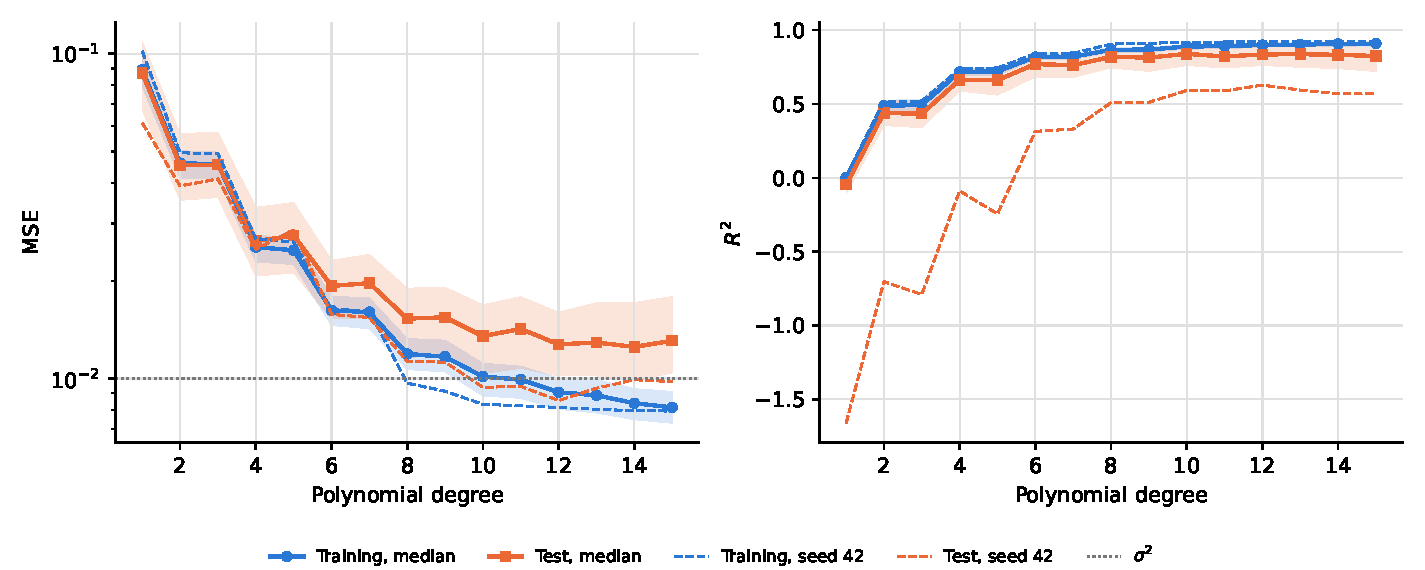
\includegraphics[width=0.85\textwidth]{a_mse_r2_degree.pdf}
    \caption{MSE (left, logarithmic) and $R^2$ (right) against polynomial degree for OLS, $n = 100$, $\sigma = 0.1$. Solid lines: median over 200 repetitions with new data and a new split each time; bands: interquartile range. Dashed lines: the single split with seed 42. Dotted line: $\sigma^2$.}
    \label{fig:a_mse_r2}
\end{figure*}

\subsubsection{How representative is one split?}

The single split (seed 42) lies below the interquartile band, and at degree 12 its test MSE, 0.0086, is even below $\sigma^2$. A test MSE below $\sigma^2$ cannot be caused by overfitting. The 20 test points happened to get less noise than average (mean squared noise $7.8\times10^{-3}$), and none of them lies at $|x| < 0.2$, around the peak. Since $f$ is known, we can compute the MSE the fitted model would get on new data: 0.0140 at degree 10, against 0.0094 on the test set. The same split gives $R^2 < 0$ up to degree 5, although its MSE there is at or below the median. The variance of $y$ in the test set is only 0.023, against 0.103 in the training set, and the same MSE divided by a four times smaller spread gives a much lower $R^2$. $R^2$ has randomness in both numerator and denominator, and its baseline is the mean of the test set itself, which a real model could not know. One small split thus makes the MSE too optimistic and $R^2$ too pessimistic, which is why we repeat the experiments, and later use resampling.

\subsubsection{Extreme repetitions and extrapolation}\label{sec:res_extreme}

At degree 15 the median test MSE is 0.013, while the mean is 0.106. Our hypothesis was that the extreme repetitions are those where a test point lies outside the interval covered by the training points, so that the high-degree polynomial must extrapolate. In 68 of 200 repetitions at least one test point lay outside, typically only a little (median distance 0.014). From degree 10, all ten worst repetitions extrapolate, and without the test points outside the training interval the mean at degree 15 drops to 0.015 (Table~\ref{tab:a_extrapolation}; see also Fig.~\ref{fig:a_extrapolation} in the appendix). At degree 20 extrapolation does not explain everything: the worst remaining repetitions have their worst test point in a gap of 0.08--0.14 in the training data, against a median spacing of 0.017, all at $|x| > 0.8$, where the prediction misses $f$ by up to 5. Inside a gap near the edge the polynomial is held from one side only and the high powers are largest. The large errors are caused by where the training points fell, not by the noise: at high degree the fit depends strongly on the particular sample.

\begin{table}
    \centering
    \caption{Test MSE over 200 repetitions ($n = 100$, $\sigma = 0.1$), with all test points and with only those inside the interval covered by the training data.}
    \label{tab:a_extrapolation}
    \begin{tabular}{rcccc}
        \toprule
        & \multicolumn{2}{c}{All test points} & \multicolumn{2}{c}{Inside} \\
        Degree & Median & Mean & Median & Mean \\
        \midrule
        5  & 0.0276 & 0.0291 & 0.0264 & 0.0278 \\
        10 & 0.0135 & 0.0151 & 0.0126 & 0.0132 \\
        15 & 0.0131 & 0.106  & 0.0123 & 0.0151 \\
        20 & 0.0155 & 19.1   & 0.0136 & 0.0361 \\
        \bottomrule
    \end{tabular}
\end{table}

\subsubsection{Dependence on the number of points and the noise}

Figure~\ref{fig:a_n_sigma} shows the median test MSE up to degree 25. Up to degree 6 the curves for all $n$ coincide: the error is dominated by bias, and more data does not help. The best degree moves up with $n$: 6, 10, 14 and 20 for $n = 30$, 50, 100 and 1000. With $n = 30$ (24 training points) the error grows quickly from about degree 12, since each extra coefficient absorbs more of the noise as the number of parameters approaches the number of training points, and the gaps are larger. With $n = 1000$ the median stays between 0.0102 and 0.0104 from degree 14 to 25: the model has reached the noise floor, and there is no clear optimum.

The best degree falls with the noise: 22, 14 and 6 for $\sigma = 0.01$, 0.1 and 0.5, and for $\sigma = 0.5$ the test error rises from degree 7. Larger $\sigma$ and smaller $n$ act in the same direction. At degree 1 the model is in practice the mean ($x$ is odd and adds nothing), and the three curves start at 0.078, 0.087 and 0.32, differing by the differences in $\sigma^2$. For $\sigma = 0.5$ the test MSE falls from 0.32 to 0.263 at degree 6 against the floor 0.25, so most of the removable error is removed. For $\sigma = 0.01$ the lowest median, $2.0\times10^{-4}$, is twice $\sigma^2$: with little noise the remaining error is mainly bias.

\begin{figure*}
    \centering
    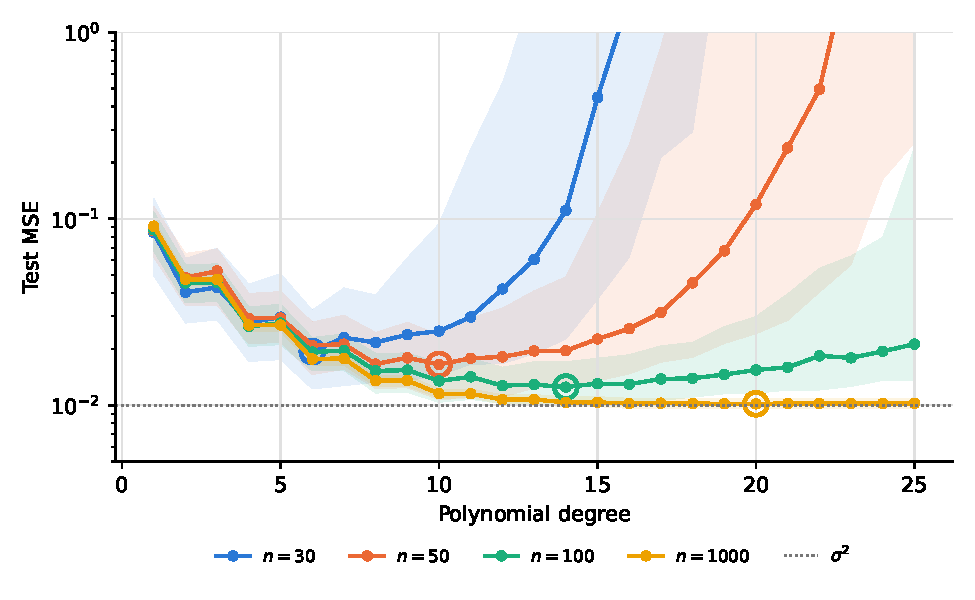
\includegraphics[width=0.49\textwidth]{a_mse_n.pdf}
    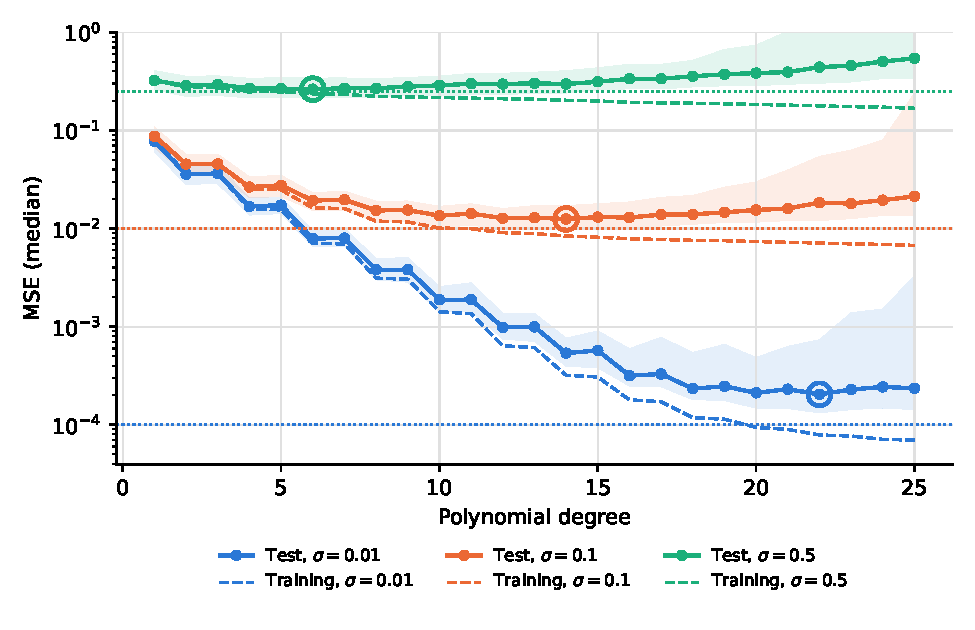
\includegraphics[width=0.49\textwidth]{a_mse_sigma.pdf}
    \caption{Median test MSE over 200 repetitions against polynomial degree. Left: $n = 30$, 50, 100 and 1000 with $\sigma = 0.1$ (dotted: $\sigma^2$). Right: $\sigma = 0.01$, 0.1 and 0.5 with $n = 100$, training (dashed) and test (solid), dotted lines at $\sigma^2$. Bands: interquartile range of the test MSE. Open circles: the degree with the lowest median.}
    \label{fig:a_n_sigma}
\end{figure*}

\subsubsection{Coefficients and scaling}\label{sec:res_scaling}

The largest $|\theta_j|$ on the standardised columns grows from 0.72 at degree 5 to 214 at degree 15 and $5\times10^{5}$ at degree 25 (Fig.~\ref{fig:a_theta}). Since all standardised columns have standard deviation 1, this is not caused by small values of $x^j$ but by collinearity: columns such as $x^{13}$ and $x^{15}$ are nearly equal on $[-1,1]$, and OLS gives them large coefficients of opposite sign that nearly cancel. The heat map shows alternating signs, and the coefficients of the low powers also grow with the degree. At degree 15 the largest odd coefficient is 214, but all odd terms together contribute at most 0.15 to the fitted curve. At high degree the individual coefficients cannot be interpreted; only the curve they form has meaning.

\begin{figure*}
    \centering
    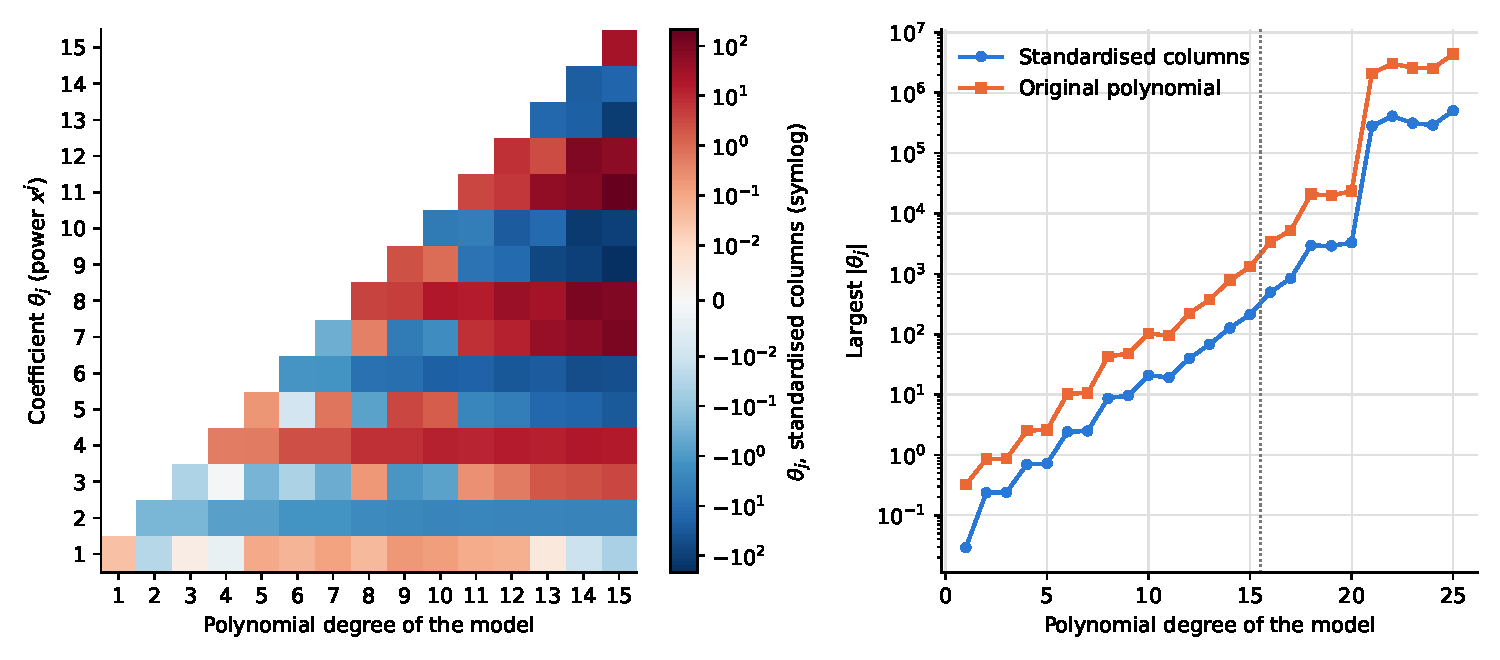
\includegraphics[width=0.85\textwidth]{a_theta_degree.pdf}
    \caption{OLS coefficients for seed 42. Left: every coefficient $\theta_j$ on the standardised columns (rows) for each model degree (columns), symmetric logarithmic colour scale. Right: the largest $|\theta_j|$ against degree, on the standardised columns and in the original polynomial; the dotted line marks the range of the left panel.}
    \label{fig:a_theta}
\end{figure*}

Table~\ref{tab:a_scaling} compares scaled and unscaled OLS on the same data. The predictions agree to $10^{-12}$ up to degree 15, since OLS compensates any rescaling of a column by rescaling its coefficient. The condition number is only halved by the scaling but grows by eight orders of magnitude with the degree: on $[-1,1]$ the powers differ little in scale, and what makes $\mathbf{X}$ ill-conditioned is the similarity of the columns, which scaling does not remove. At degree 25 ($\kappa \approx 10^9$) round-off shows as a difference of $2\times10^{-7}$ between the two solutions. For OLS on this data set scaling is therefore not needed. It would matter more on a wider interval such as $[-3, 3]$ or with features in different units. The growing condition number is the problem Ridge addresses.

\begin{table}
    \centering
    \caption{Scaled against unscaled OLS (seed 42). Unscaled: column of ones kept, no centering. $\kappa$: condition number of the training design matrix. $\Delta$: largest difference between the two predictions on the test points.}
    \label{tab:a_scaling}
    \begin{tabular}{rccc}
        \toprule
        & \multicolumn{2}{c}{$\kappa(\mathbf{X})$} & \\
        Degree & Scaled & Unscaled & $\Delta$ \\
        \midrule
        5  & 25                 & 48                 & $2\times10^{-14}$ \\
        10 & $1.7\times10^{3}$  & $3.8\times10^{3}$  & $3\times10^{-14}$ \\
        15 & $1.6\times10^{5}$  & $3.5\times10^{5}$  & $7\times10^{-13}$ \\
        20 & $1.6\times10^{7}$  & $3.6\times10^{7}$  & $1\times10^{-10}$ \\
        25 & $2.7\times10^{9}$  & $6.1\times10^{9}$  & $2\times10^{-7}$  \\
        \bottomrule
    \end{tabular}
\end{table}

\subsection{Ridge regression}\label{sec:res_ridge}

\subsubsection{Shrinkage of the singular-value directions}

Figure~\ref{fig:b_svd} connects Ridge to the singular values of our own design matrix (degree 15, seed 42). The squared singular values fall from 783 to $3\times10^{-8}$ (panel 1). The smallest ones come from collinearity between the high powers and are the flat directions of the cost. Each Ridge penalty $n\lambda$ is a horizontal line in panel 1, and where $\sigma_i^2$ crosses it the shrinkage factor in panel 2 is $1/2$. For $\lambda = 10^{-2}$ ($n\lambda = 0.8$) the crossing lies between directions 6 and 7; the factor is 0.87 for direction 5, 0.33 for direction 7, 0.09 for direction 8, and practically zero from direction 10. The smaller penalties show the same pattern for later directions.

Panel 3 shows how much of the data lies in each pattern $\mathbf{u}_i$. For the first ten directions $|\mathbf{u}_i^T\mathbf{y}|$ is between 0.4 and 1.6, while from direction 11 it lies at the noise level $\sigma = 0.1$: in the flattest directions the data contain practically only noise. Panel 4 shows the consequence. OLS divides this noise by the tiny $\sigma_i$, and the component of $\hat{\boldsymbol{\theta}}$ along $\mathbf{v}_i$ grows from 0.03 to 288; the large components are amplified noise, i.e.\ the variance from Sec.~\ref{sec:res_ols}. Ridge multiplies each component by its shrinkage factor, which we can read off directly: for $\lambda = 10^{-2}$ a third remains in direction 7 and a tenth in direction 8. Ridge thus removes mainly directions that contain noise, which is why it can reduce the variance much at a small cost in bias. For a large penalty it also removes directions with real signal: with $\lambda = 10^{-2}$ directions 6--8 have $|\mathbf{u}_i^T\mathbf{y}|$ between 0.45 and 1.0, well above the noise, and are strongly shrunk.

\begin{figure*}
    \centering
    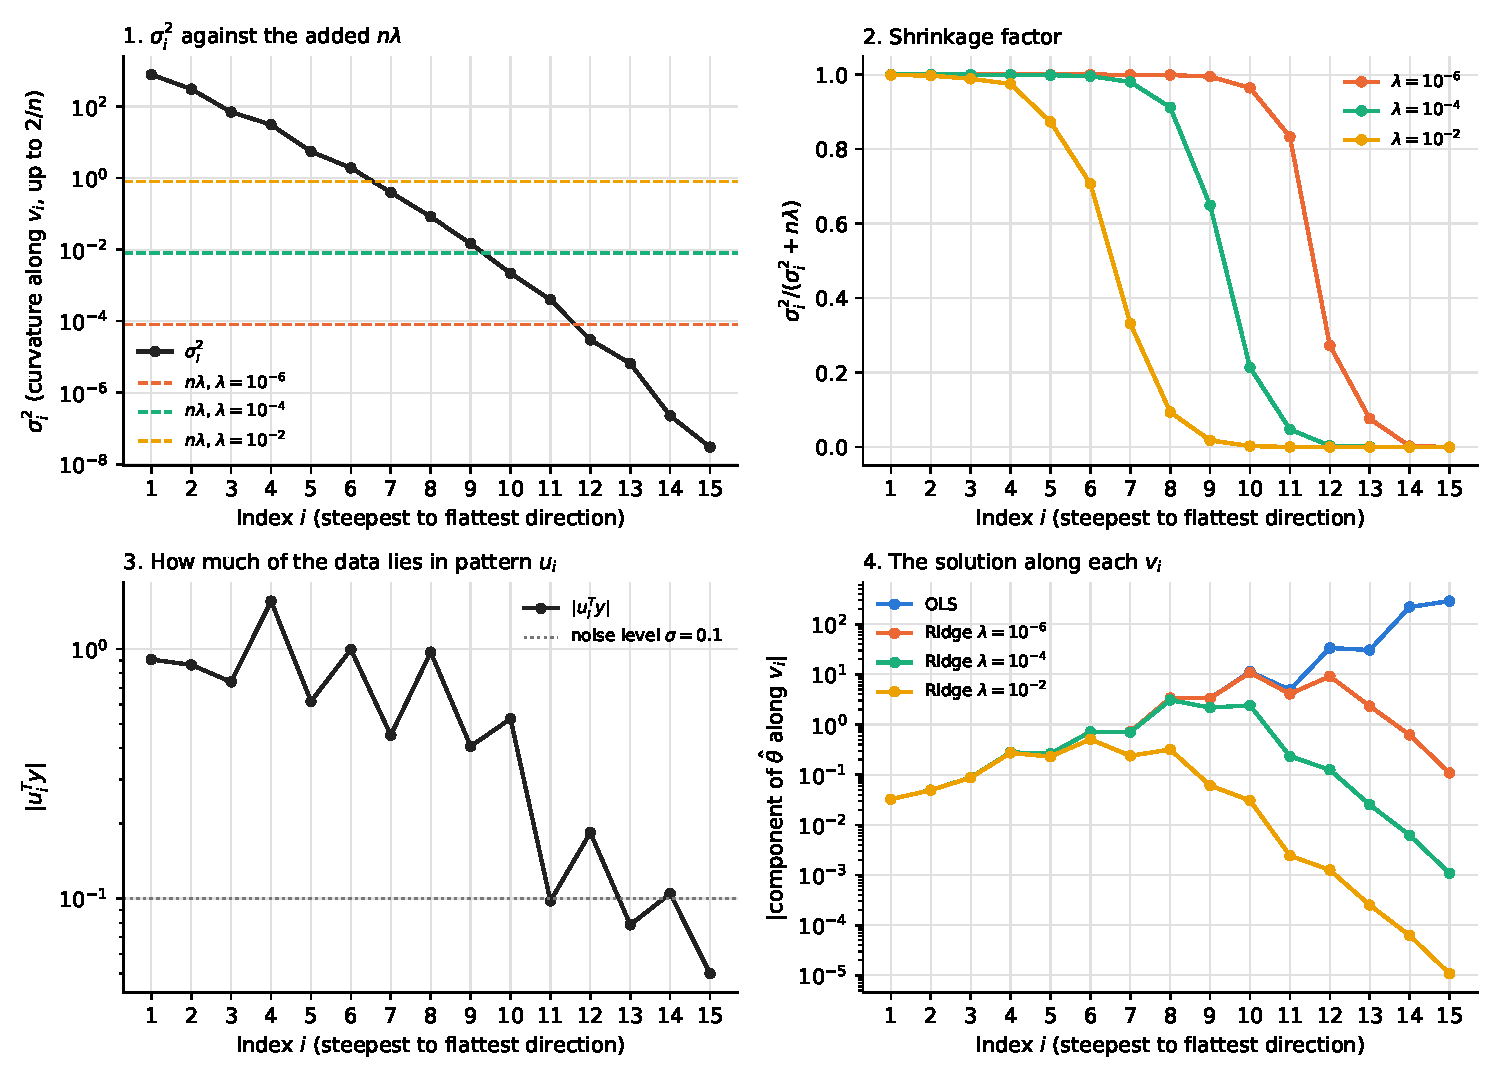
\includegraphics[width=0.8\textwidth]{b_svd_shrinkage.pdf}
    \caption{Singular-value analysis of the standardised design matrix, degree 15, seed 42, $n_{\mathrm{train}} = 80$. 1: $\sigma_i^2$ with the penalty $n\lambda$ for three values of $\lambda$. 2: the shrinkage factor $\sigma_i^2/(\sigma_i^2+n\lambda)$. 3: $|\mathbf{u}_i^T\mathbf{y}|$, how much of the (centred) training data lies in pattern $\mathbf{u}_i$, with the noise level $\sigma$. 4: the component of $\hat{\boldsymbol{\theta}}$ along $\mathbf{v}_i$ for OLS and Ridge.}
    \label{fig:b_svd}
\end{figure*}

\subsubsection{Error against degree and penalty}

Figures~\ref{fig:b_mse_r2} and \ref{fig:b_heatmap} show the test error for Ridge. With $n = 100$ Ridge does not improve on the best OLS model: the lowest median over all degrees and penalties is OLS at degree 14 (0.0125); $\lambda = 10^{-6}$ is close (0.0133 at degree 10), while $\lambda = 10^{-2}$ gives 0.026. With $\lambda = 10^{-2}$ the shrinkage removes real signal (above), which is bias. What Ridge changes is the behaviour away from the optimum. The Ridge curves do not rise at high degree, and their interquartile bands stay narrow, because the directions that let the curve swing in gaps and at the edges are removed. The means show the same: at degree 20 the mean test MSE is 19 for OLS, 0.037 for $\lambda = 10^{-6}$ and 0.021 for $\lambda = 10^{-4}$. Ridge does not make a good model better, but it makes the result much less sensitive to a poor choice of complexity, which matters because the right degree is not known in practice.

With $n = 30$ the difference is larger (right panel of Fig.~\ref{fig:b_heatmap}). The best median is now a Ridge model, $\lambda \approx 3\times10^{-5}$ at degree 8 (0.0187, against 0.0194 for OLS at degree 6), and OLS explodes from about degree 14, while the rows with small and moderate penalties stay between 0.02 and 0.05. With fewer points there is more noise per parameter, and the penalty pays off more, in line with the dependence on $n$ in Sec.~\ref{sec:res_ols}. The heat map shows medians. The means reveal that a small penalty does not fully protect against the extreme repetitions: at degree 10 the mean test MSE is 3.1 for $\lambda = 10^{-6}$, 0.41 for $\lambda = 10^{-4}$ and 0.044 for $\lambda = 10^{-2}$.

For large penalties the rows of the heat map become nearly uniform. At $\lambda = 10$ and $n = 100$ the median test MSE is 0.073--0.087 at all degrees, close to the degree-1 model, which in practice predicts the mean: the penalty has pushed all coefficients towards zero, and the error is dominated by bias.

\begin{figure*}
    \centering
    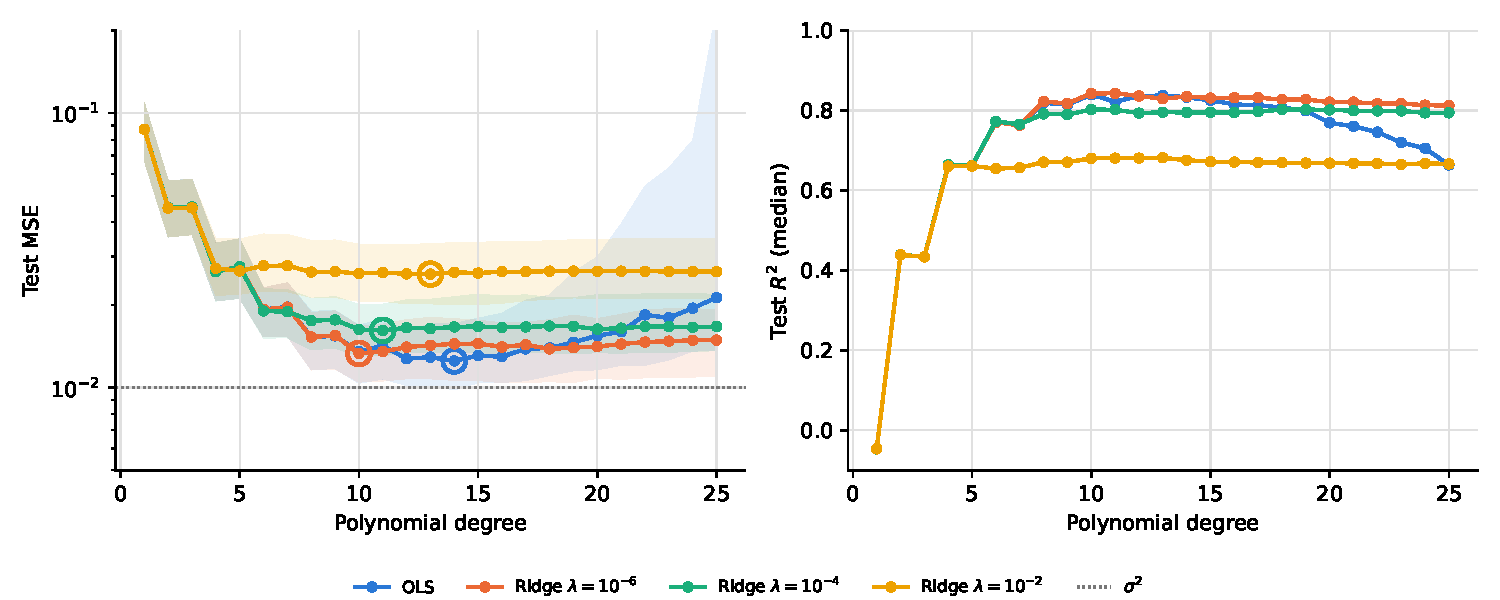
\includegraphics[width=0.85\textwidth]{b_mse_r2_degree.pdf}
    \caption{Test MSE (left, logarithmic) and median test $R^2$ (right) against degree for OLS and Ridge with three penalties, $n = 100$, $\sigma = 0.1$, 200 repetitions. Bands: interquartile range. Open circles: the degree with the lowest median. Dotted line: $\sigma^2$.}
    \label{fig:b_mse_r2}
\end{figure*}

\begin{figure*}
    \centering
    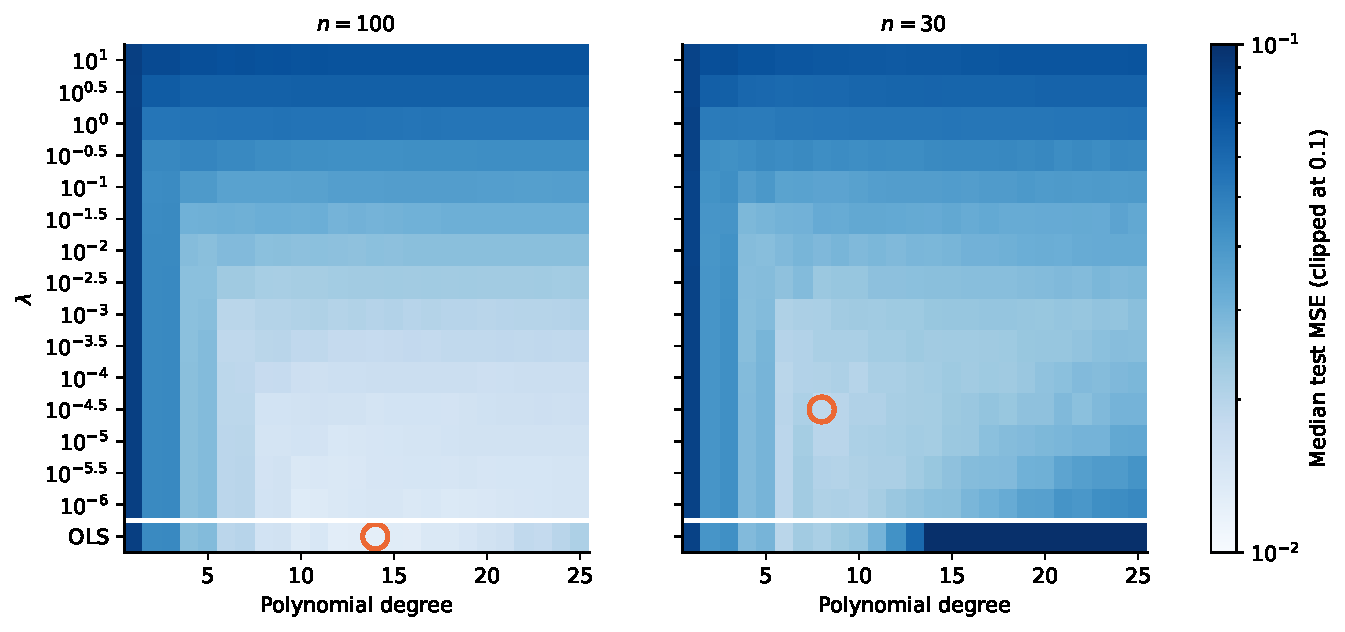
\includegraphics[width=0.85\textwidth]{b_heatmap.pdf}
    \caption{Median test MSE over 200 repetitions against degree and penalty, $n = 100$ (left) and $n = 30$ (right), $\sigma = 0.1$. The bottom row is OLS. Colours are clipped at 0.1. Circle: the lowest median.}
    \label{fig:b_heatmap}
\end{figure*}

\subsubsection{Coefficients}

Figure~\ref{fig:b_theta} repeats the coefficient plot of Fig.~\ref{fig:a_theta} for Ridge. While the largest OLS coefficient keeps growing with the degree, the Ridge coefficients level off at about 10, 3.5 and 0.63 for $\lambda = 10^{-6}$, $10^{-4}$ and $10^{-2}$. The penalty lifts the flat directions along which the OLS solution can wander when it fits noise. Once the directions added by a higher degree have $\sigma_i^2 \ll n\lambda$ they are shrunk to nothing, so a larger penalty makes the curve level off at a lower degree and a lower value.

\begin{figure}
    \centering
    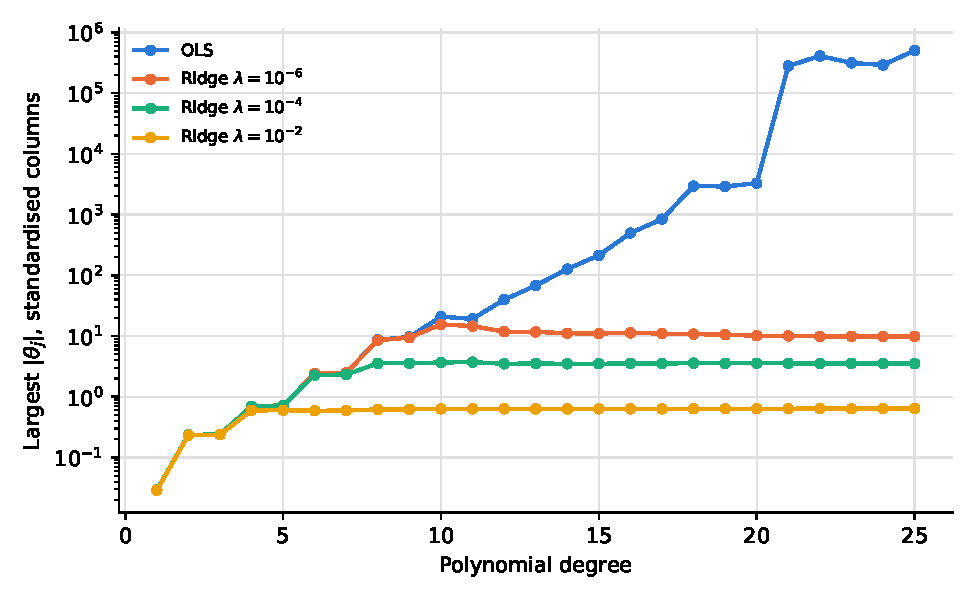
\includegraphics[width=\linewidth]{b_theta_degree.pdf}
    \caption{Largest $|\theta_j|$ on the standardised columns against degree for OLS and Ridge (seed 42).}
    \label{fig:b_theta}
\end{figure}

\subsection{Bias--variance trade-off with the bootstrap}\label{sec:res_bootstrap}

Figure~\ref{fig:c_train_test} shows training and test MSE against degree for $n = 50$, in the style of Fig.~2.11 of Hastie \textit{et al.} \cite{Hastie2009}. The training MSE falls monotonically and is below $\sigma^2$ from degree 8. The test MSE has its minimum at degrees 8--10 (0.017) and rises to 0.12 at degree 20 and 39 at degree 25. To the left of the minimum the error is dominated by bias, to the right by variance.

\begin{figure}
    \centering
    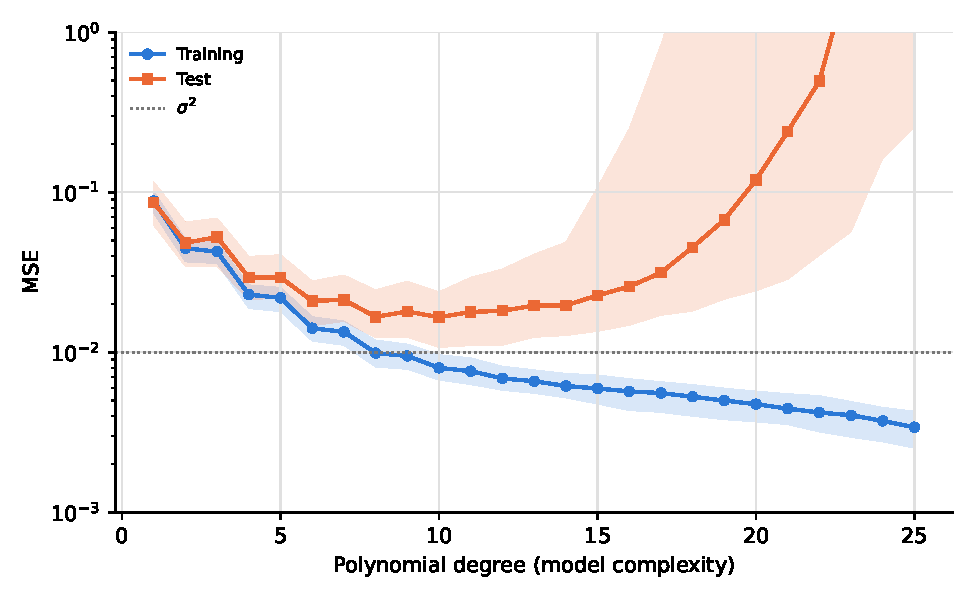
\includegraphics[width=\linewidth]{c_train_test.pdf}
    \caption{Training and test MSE against polynomial degree for OLS, $n = 50$, $\sigma = 0.1$. Median over 200 repetitions; bands: interquartile range. Dotted line: $\sigma^2$.}
    \label{fig:c_train_test}
\end{figure}

Figure~\ref{fig:c_bias_variance} shows the bootstrap decomposition for $n = 50$, 100 and 400. For $n = 100$ the squared bias falls from 0.093 at degree 1 to about 0.015 at degree 8 and then stays between 0.014 and 0.018 up to degree 14. The variance is 0.002--0.004 up to degree 8 and then grows by two orders of magnitude, to 0.31 at degree 14. It exceeds the squared bias from degree 11, and the error has its minimum at degree 8 (0.019). With $n = 50$ the variance takes over already at degree 7 and the minimum is at degree 4; the curves are jagged because of the odd and even degrees and the small test set. With $n = 400$ the variance stays below $9\times10^{-4}$ at all degrees, never exceeds the bias, and the error decreases to 0.011 at degree 15. More data thus moves the point where variance takes over to higher degree, in line with Sec.~\ref{sec:res_ols}.

The dashed lines show the squared bias measured against $f$ instead of $y$. For $n = 100$ and 400 the difference between the two is 0.009--0.011 at all degrees where the variance is small, i.e.\ $\sigma^2$: the measured bias absorbs the noise, as expected from Sec.~\ref{sec:biasvar}. The bias measured against $f$ keeps falling with the degree (to $9\times10^{-4}$ at degree 14 for $n = 400$), while the measured bias stops at the noise floor. At high degree and small $n$ the measured bias also grows, because the mean of the 100 bootstrap predictions is itself pulled away by a few extreme fits.

\begin{figure*}
    \centering
    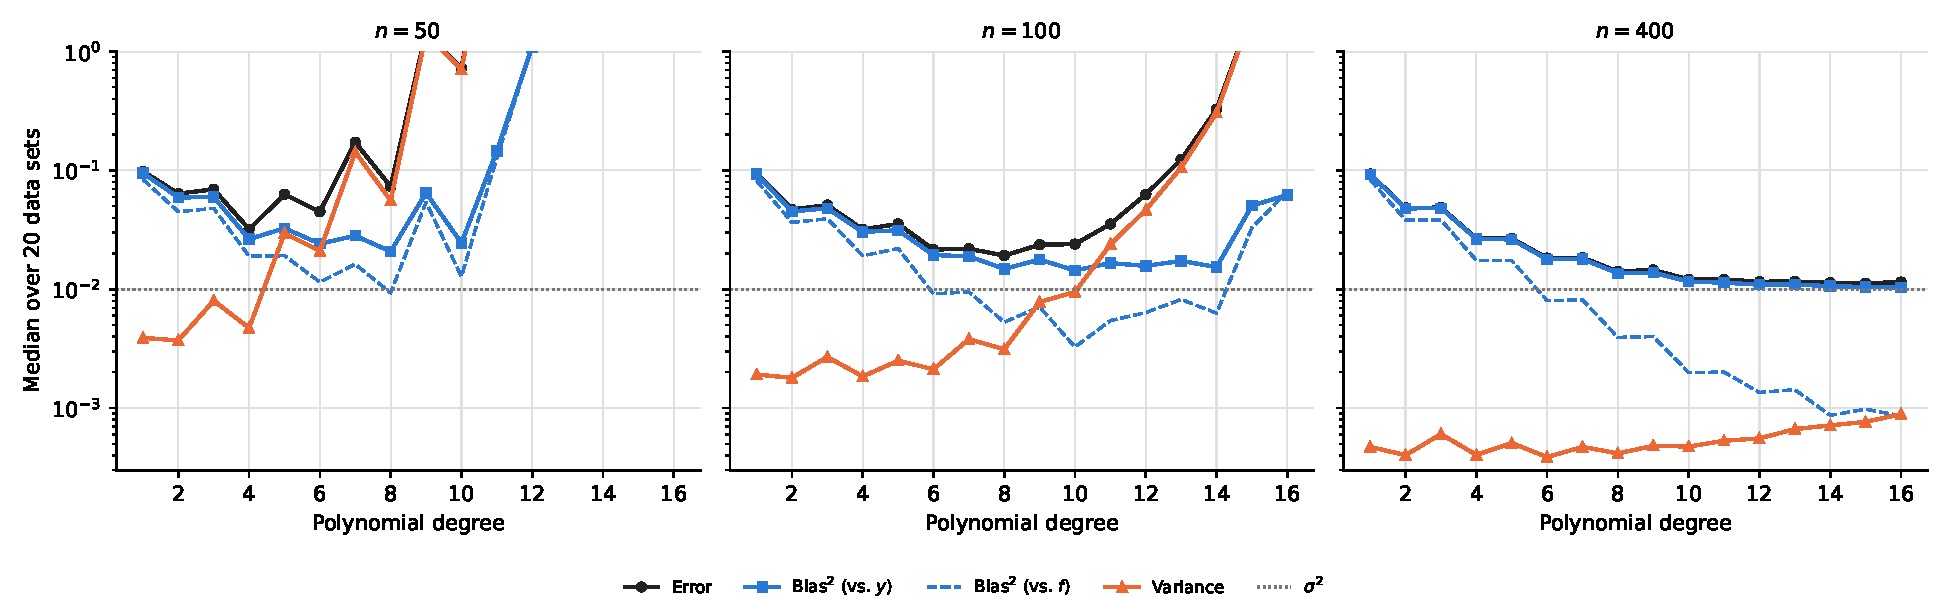
\includegraphics[width=\textwidth]{c_bias_variance.pdf}
    \caption{Bootstrap estimates of the test error, squared bias and variance against degree for OLS, $n = 50$, 100 and 400, $\sigma = 0.1$, 100 bootstrap samples; median over 20 data sets. Solid bias: measured against $y$; dashed: against the true $f$. Dotted line: $\sigma^2$.}
    \label{fig:c_bias_variance}
\end{figure*}

\subsection{Cross-validation}\label{sec:res_cv}

Figure~\ref{fig:d_cv} compares cross-validation with the bootstrap test error and with the MSE on new data for $n = 100$. Cross-validation follows the reference closely, slightly above it (at degree 10: 0.0144 for $k = 5$, 0.0142 for $k = 10$, 0.0133 on new data). It points to degree 11 ($k = 5$) or 14 ($k = 10$), against 12 for the reference; the curves are nearly flat from degree 10 to 16, so the exact minimum is not well determined. The difference between $k = 5$ and $k = 10$ is small; with $k = 10$ each model is trained on 90 instead of 80 points, which gives a slightly lower error at high degree.

The bootstrap agrees with the other two up to degree 7, but then overestimates the error strongly (0.063 at degree 12, against 0.013 on new data) and points to degree 8. The two methods therefore do not point to the same complexity. The reason is that a bootstrap sample drawn with replacement contains on average only about 63\,\% distinct points ($1 - 1/e$), so each model is fitted on about 50 distinct points instead of 80. The variance grows earlier with the degree, as for a smaller $n$ in Sec.~\ref{sec:res_ols}. The bootstrap is well suited to split the error into bias and variance, while cross-validation, which uses all points for both fitting and validation, gives the better estimate of the error for model selection.

\begin{figure}
    \centering
    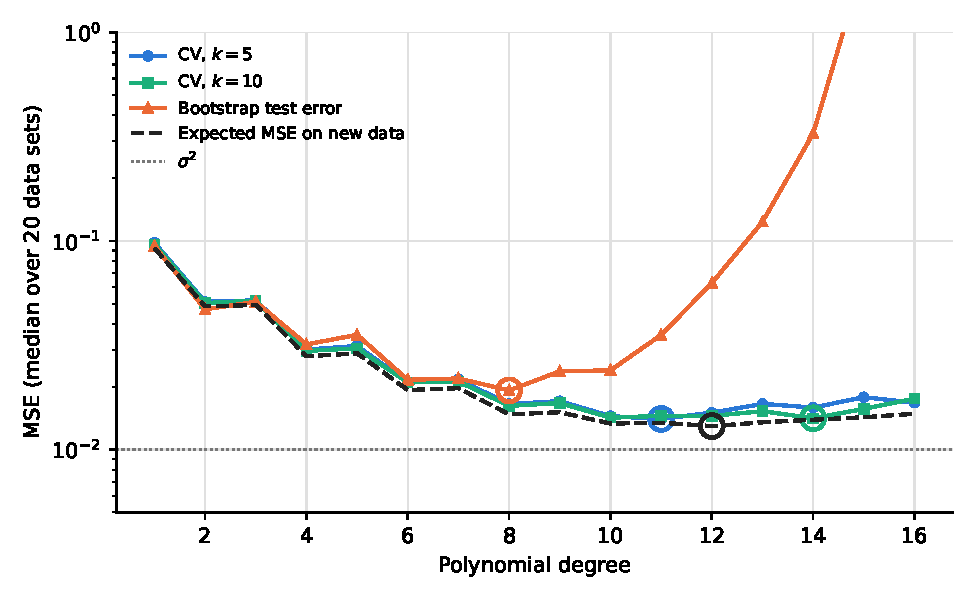
\includegraphics[width=\linewidth]{d_cv_vs_bootstrap.pdf}
    \caption{OLS: cross-validation MSE ($k = 5$ and 10), bootstrap test error and the MSE on new data against degree, $n = 100$, $\sigma = 0.1$; median over 20 data sets. Open circles: lowest value of each curve.}
    \label{fig:d_cv}
\end{figure}

For Ridge (Fig.~\ref{fig:d_cv_ridge}) the lowest cross-validation error is at degree 11 with $\lambda = 3\times10^{-8}$ (0.0139), practically the same as OLS at the same degree (0.0140). With $n = 100$ the penalty gives no gain at the best degree, as in Sec.~\ref{sec:res_ridge}, but it does at high degree: at degree 15 the best penalty, $\lambda = 3\times10^{-7}$, gives 0.0148 against 0.0178 for OLS. Large penalties give a high error at all degrees (bias).

\begin{figure}
    \centering
    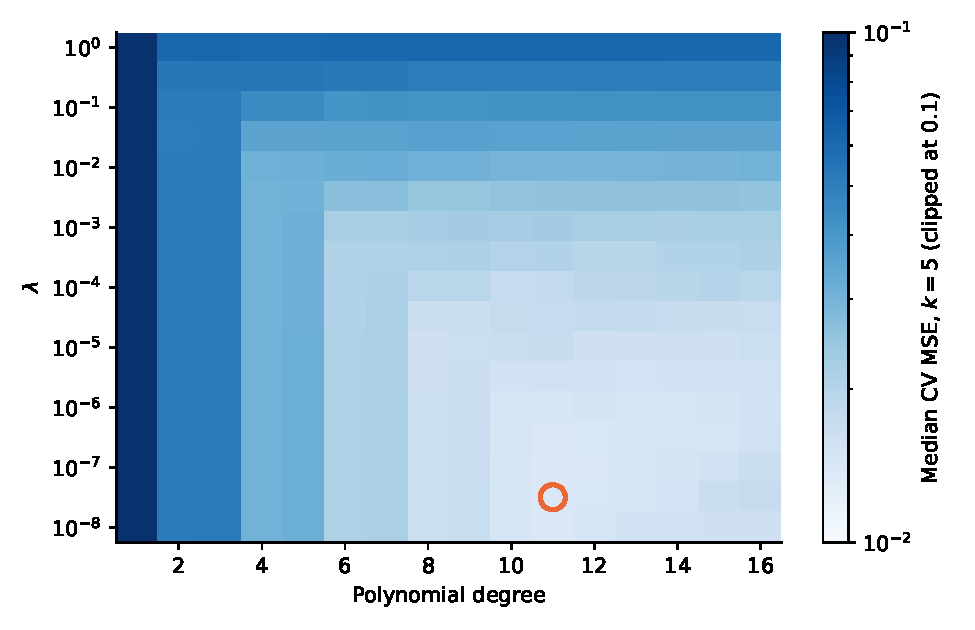
\includegraphics[width=\linewidth]{d_cv_ridge.pdf}
    \caption{Ridge: median 5-fold cross-validation MSE over 20 data sets against degree and $\lambda$, $n = 100$, $\sigma = 0.1$. Colours clipped at 0.1. Circle: the lowest value.}
    \label{fig:d_cv_ridge}
\end{figure}

\subsection{Gradient descent with a fixed learning rate}\label{sec:res_gd}

The analytic gradient and the JAX gradient agree to $2\times10^{-16}$ for both OLS and Ridge, and 2000 gradient-descent iterations with either gradient give coefficients that differ by at most $2\times10^{-15}$. On a larger problem ($10^5 \times 50$) one reverse-mode gradient took 2.6 times as long as one evaluation of the cost (between 2.4 and 3.1 in repeated runs), in line with the statement that the gradient costs a small multiple of the function.

For OLS at degree 6 the Hessian eigenvalues range from $3.4\times10^{-3}$ to 7.63 ($\kappa = 2.3\times10^3$), so $\gamma_{\max} = 2/\mu_{\max} = 0.262$. Figure~\ref{fig:e_gd} shows that gradient descent converges to the closed-form solution for every $\gamma < \gamma_{\max}$ and diverges just above it: at $1.01\,\gamma_{\max}$ the coefficients blow up within about 1100 iterations. The number of iterations to $\lVert\boldsymbol{\theta} - \hat{\boldsymbol{\theta}}\rVert < 10^{-6}$ falls from 336\,841 at $0.05\,\gamma_{\max}$ to 16\,843 at $\gamma^*$, and agrees within 0.5\,\% with the prediction from the slowest mode, $\ln(\lVert\hat{\boldsymbol{\theta}}\rVert/10^{-6}) / (-\ln\max_i|1 - \gamma\mu_i|)$. For Ridge the prediction is 4\,\% too high, since it counts the whole initial distance $\lVert\hat{\boldsymbol{\theta}}\rVert$ as lying along the slowest mode. The slow convergence is caused by the flat direction ($\mu_{\min}$), while the largest usable learning rate is set by the steepest ($\mu_{\max}$). Ridge with $\lambda = 10^{-2}$ raises $\mu_{\min}$ to 0.023 ($\kappa = 327$) and needs about eight times fewer iterations (2138 at $0.99\,\gamma_{\max}$). The converged solutions reproduce the closed-form test MSE to six digits (0.015751 for OLS, 0.024435 for Ridge).

\begin{figure*}
    \centering
    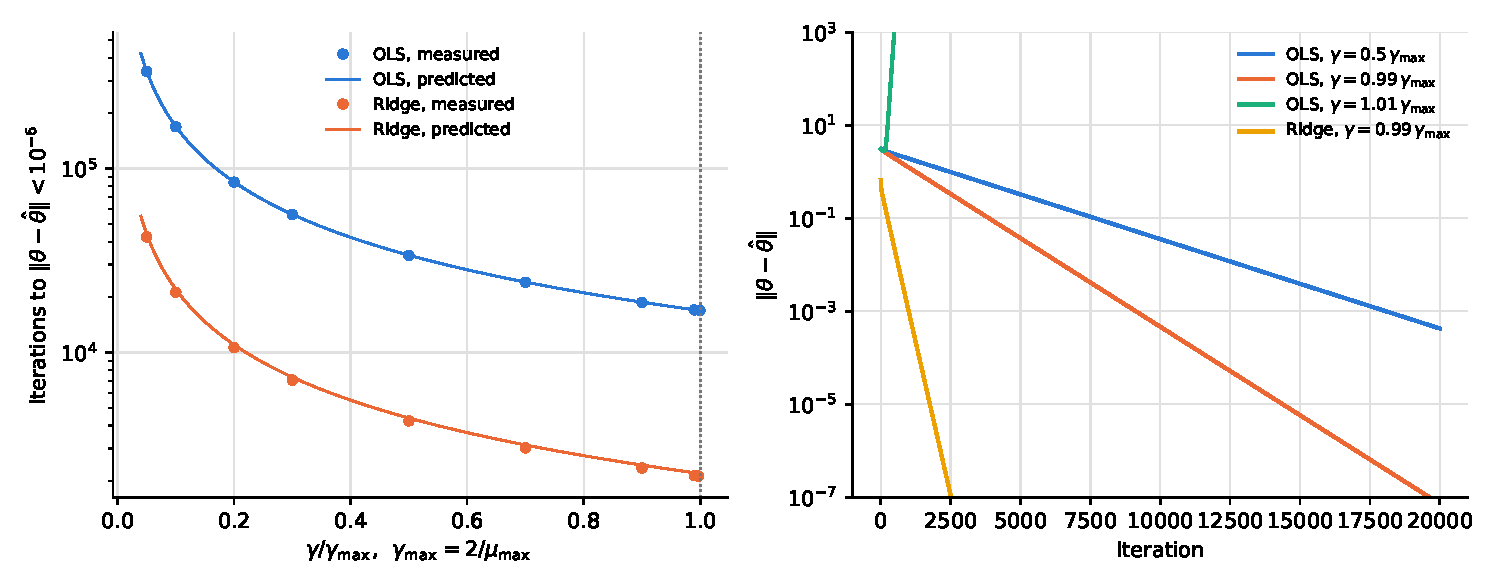
\includegraphics[width=0.85\textwidth]{e_gd.pdf}
    \caption{Plain gradient descent, degree 6, seed 42. Left: iterations to reach $\lVert\boldsymbol{\theta} - \hat{\boldsymbol{\theta}}\rVert < 10^{-6}$ against the learning rate relative to $\gamma_{\max} = 2/\mu_{\max}$, measured (points) and predicted from the Hessian eigenvalues (lines), for OLS and Ridge ($\lambda = 10^{-2}$). Right: distance to the closed-form solution against iteration.}
    \label{fig:e_gd}
\end{figure*}

\subsection{Momentum and adaptive learning rates}\label{sec:res_adaptive}

Figure~\ref{fig:f_methods} shows the number of iterations needed to bring the cost within $10^{-8}$ of the closed-form minimum, against the (initial) learning rate, for the same problem as in Sec.~\ref{sec:res_gd}. The criterion is now on the cost rather than on the distance to $\hat{\boldsymbol{\theta}}$ as in Sec.~\ref{sec:res_gd}; in a flat direction a large distance costs little, and the cost is what matters for the predictions. For OLS plain gradient descent converges within $10^5$ iterations for $\gamma$ from 0.032 to 0.178, the largest value in our grid below $\gamma_{\max} = 0.262$, and the number of iterations falls as $1/\gamma$, from 66\,559 to 11\,834. Momentum is the fastest method: 601 iterations at best, 20 times fewer than plain gradient descent, and it converges for $\gamma$ from 0.0032 to 0.32. AdaGrad converges for $\gamma \geq 0.018$ but needs at least 13\,786 iterations, and below $\gamma = 0.1$ the number rises steeply (92\,163 at $\gamma = 0.018$), since the sum of squared gradients only grows and the steps keep shrinking. Adam needs 842 iterations at best, but its main advantage is robustness: it reaches the criterion for all 17 learning rates from $10^{-4}$ to 1, and from $\gamma \approx 0.06$ the number of iterations hardly changes (842--1135). Since it divides by the running size of the gradient, a large gradient does not give a large step, and a too large $\gamma$ does not make it diverge as plain gradient descent does. With Ridge ($\lambda = 10^{-2}$) all methods that converge are faster, as in Sec.~\ref{sec:res_gd}, since the flattest direction is lifted: 138 iterations for momentum, 174 for Adam and 1475 for plain gradient descent.

The adaptive methods rescale each coefficient separately, but the flat direction of this problem is a combination of nearly collinear columns, not a coordinate axis (Sec.~\ref{sec:adaptive}). They therefore do not remove the ill-conditioning; momentum, which builds up speed along the valley floor, gives the largest gain.

RMSProp never reaches the criterion. Every coefficient ends in a cycle, jumping between two points $\gamma/2$ on either side of the optimum: when the size of the gradient is constant, the running mean $r$ equals $g^2$, and the step $\gamma g/\sqrt{r}$ is exactly $\gamma$, however small the gradient is. The remaining excess cost therefore grows as $\gamma^2$: $5.7\times10^{-8}$, $5.7\times10^{-6}$ and $5.7\times10^{-4}$ for $\gamma = 10^{-4}$, $10^{-3}$ and $10^{-2}$. Adam reaches the criterion but does not stay there: with $\gamma = 0.056$ the excess cost repeatedly jumps to between $3.8\times10^{-3}$ and $5.3\times10^{-3}$ from iteration 1465 on (right panel). Adam divides the step by a running average of the size of earlier gradients. Near the minimum the gradients are small, this average shrinks slowly, and the steps therefore become gradually longer. In the end they become too long, as for plain gradient descent with $\gamma$ above $\gamma_{\max}$, and the deviation grows quickly until the larger gradients make the steps shorter again. We checked that the steps pass the stability limit shortly before the first jump, at iteration 1366. A smaller $\gamma$ gives smaller jumps ($\gamma = 10^{-3}$ does not exceed $1.3\times10^{-6}$ in the last 1000 iterations), but needs more iterations.

\begin{figure*}
    \centering
    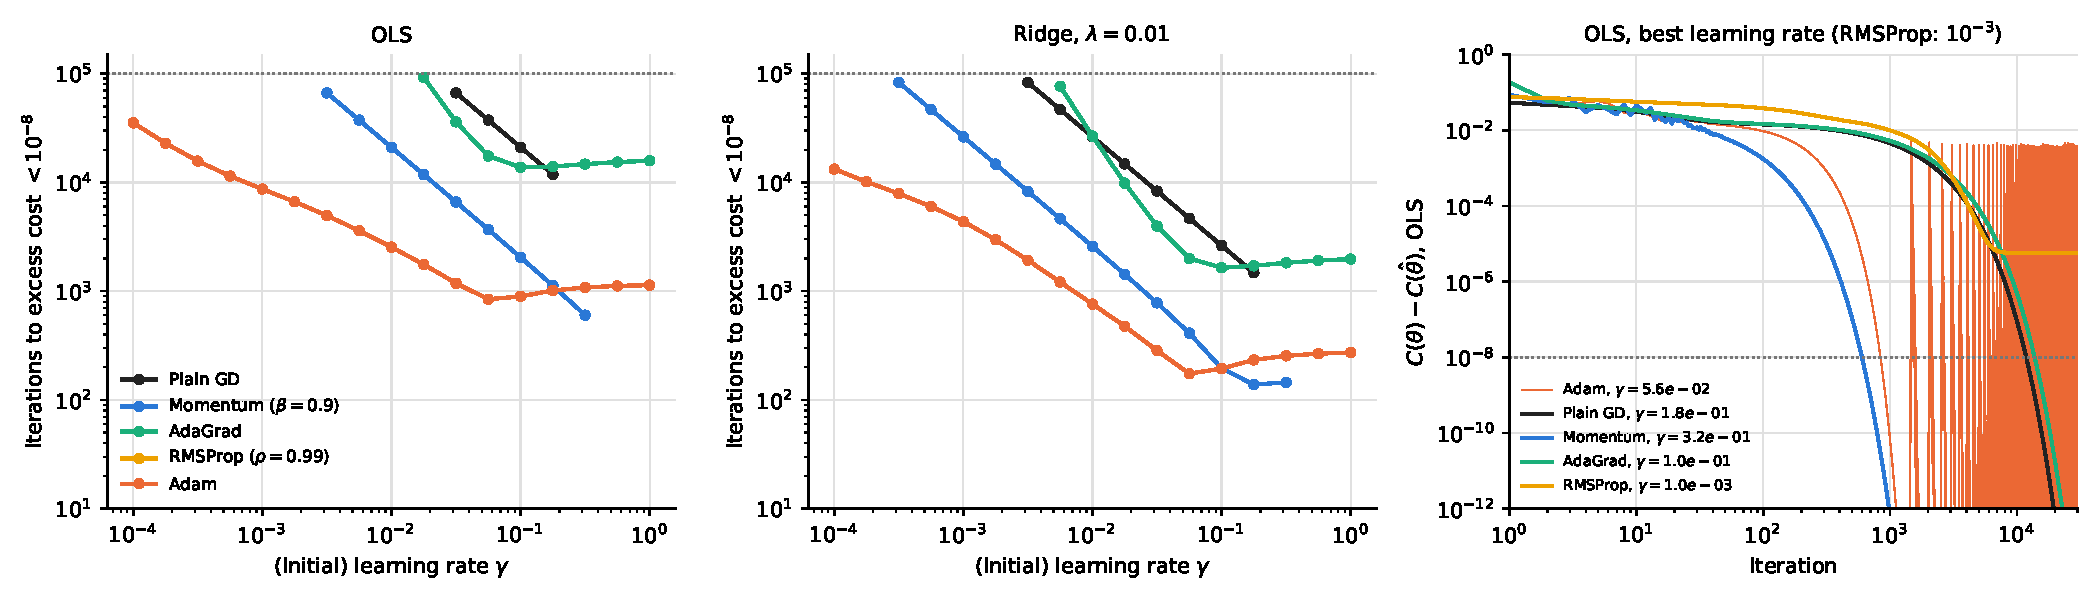
\includegraphics[width=\textwidth]{f_methods.pdf}
    \caption{Degree 6, seed 42, start at $\boldsymbol{\theta} = 0$. Left and middle: iterations until the cost is within $10^{-8}$ of the closed-form minimum against the (initial) learning rate, for OLS and Ridge ($\lambda = 10^{-2}$); missing points did not reach it within $10^5$ iterations (RMSProp never does). Right: excess cost against iteration for OLS at each method's best learning rate (RMSProp at $10^{-3}$), first $3\times10^4$ iterations.}
    \label{fig:f_methods}
\end{figure*}

\subsection{Lasso}\label{sec:res_lasso}

JAX returns $\mathrm{d}|\theta|/\mathrm{d}\theta = 1$ at $\theta = 0$ (also at $-0$), a valid subgradient. For $\lambda = 10^{-4}$ and $10^{-3}$ no coefficient is zero at the optimum, and both plain gradient descent and Adam reproduce scikit-learn's solution (cost difference below $10^{-8}$). For $\lambda = 10^{-2}$ scikit-learn sets $\theta_5$ and $\theta_6$ exactly to zero, and the optimality condition holds ($|\frac{2}{n}\mathbf{x}_j^T\mathbf{r}| = 4.8\times10^{-3}$ and $3.9\times10^{-3}$, below $\lambda$). Gradient descent never produces exact zeros. Where a coefficient is zero at the optimum, the cost has a kink, and the slope does not become smaller close to the kink; with a fixed $\gamma$ the steps therefore do not shrink, and gradient descent keeps jumping across it. Adam comes to within about $1.5\times10^{-6}$ of the optimal cost (smallest $|\theta_j| = 3\times10^{-5}$). Plain gradient descent at $0.99\,\gamma_{\max}$, where it is barely stable, fails: the excess cost stays at 0.12--0.13, and four of the six coefficients changed sign in the last step. A smaller step gives smaller jumps (Table~\ref{tab:g_lasso}), but a fixed-step subgradient method never settles exactly; a decreasing step, or a method that sets coefficients exactly to zero, as scikit-learn's coordinate descent does, is needed.

\begin{table}
    \centering
    \caption{Plain subgradient descent for Lasso (analytic subgradient, $\mathrm{sign}(0) = 0$), $\lambda = 10^{-2}$, degree 6: smallest and largest excess cost over scikit-learn's solution in the last 1000 of $10^5$ iterations, for four fixed learning rates.}
    \label{tab:g_lasso}
    \begin{tabular}{cc}
        \toprule
        $\gamma / \gamma_{\max}$ & Excess cost \\
        \midrule
        0.99 & 0.12--0.13 \\
        0.90 & $5.8\times10^{-4}$--$1.6\times10^{-3}$ \\
        0.50 & $2.1\times10^{-6}$--$3.4\times10^{-5}$ \\
        0.10 & $8.3\times10^{-8}$--$4.5\times10^{-6}$ \\
        \bottomrule
    \end{tabular}
\end{table}

Figure~\ref{fig:g_lasso} shows the Lasso path from scikit-learn with the gradient-descent solutions. As $\lambda$ grows the coefficients shrink and more of them become exactly zero: none at $\lambda = 10^{-3}$, $\theta_5$ and $\theta_6$ at $10^{-2}$, and at $0.1$ only the $x^2$ term is left. The odd powers are small for all $\lambda$, as expected for an even function. On the test set (seed 42) Lasso with $\lambda = 10^{-4}$ and $10^{-3}$ is nearly as good as OLS (0.0158 and 0.0162 against 0.0158); with $\lambda = 10^{-2}$ the error rises to 0.024, like Ridge with the same $\lambda$ (0.024). At degree 6 there is little variance to remove, so neither penalty helps here.

\begin{figure}
    \centering
    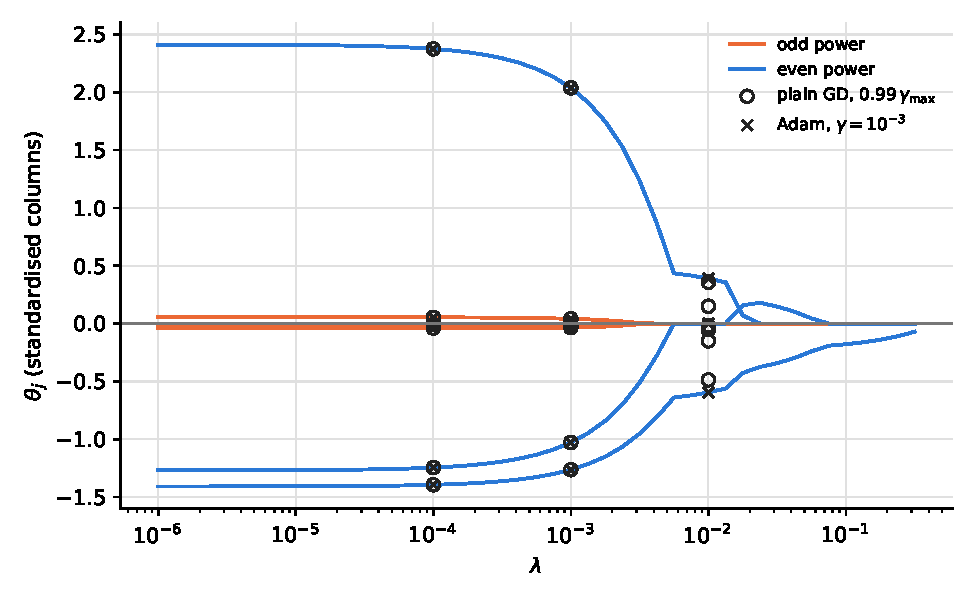
\includegraphics[width=\linewidth]{g_lasso_path.pdf}
    \caption{Lasso coefficients on the standardised columns against $\lambda$, degree 6, seed 42. Lines: scikit-learn (blue: even powers, orange: odd powers). Markers: gradient descent with the JAX subgradient at $\lambda = 10^{-4}$, $10^{-3}$ and $10^{-2}$, plain with $\gamma = 0.99\,\gamma_{\max}$ (circles) and Adam with $\gamma = 10^{-3}$ (crosses); at $\lambda = 10^{-2}$ plain gradient descent misses the path.}
    \label{fig:g_lasso}
\end{figure}

\subsection{Stochastic gradient descent}\label{sec:res_sgd}

Figure~\ref{fig:h_sgd} shows the training cost above the closed-form minimum against epochs. With plain SGD and a constant $\gamma = 0.05$, smaller batches, down to $M = 5$, give more updates per epoch and faster progress, and $M = 5$ reaches the lowest cost after 1000 epochs ($1.7\times10^{-4}$, test MSE 0.0164 against 0.0158 for the closed form). $M = 1$ is too noisy: $\gamma = 0.05$ is above the stability limit $2/(2\lVert\mathbf{x}_i\rVert^2)_{\max} = 0.018$ for single points, and the cost fluctuates at about $10^{-2}$ or higher ($1.2\times10^{-2}$ after 100 and $1.8\times10^{-2}$ after 1000 epochs; test MSE 0.058). With $M = 80$ plain SGD is full-batch gradient descent with a small step and is slow. We therefore used $M = 5$ for the comparison of the update rules. The schedule $\gamma_t = 50/(t + 500)$ decays too fast when $t$ counts updates (16 per epoch): after 1000 epochs $\gamma_t = 0.003$, and the cost is $4.6\times10^{-3}$, against $1.7\times10^{-4}$ with the constant $\gamma = 0.05$.

Measured in passes through the data, SGD reaches a moderate accuracy about as fast as full-batch gradient descent with the same update rule, or faster. An excess cost of $10^{-3}$ takes 269 epochs with SGD and momentum and 333 with SGD and Adam, against 397 and 315 iterations for full-batch momentum and Adam, and plain SGD gets there after 523 epochs, while full-batch plain gradient descent is still at $2.6\times10^{-3}$ after 1000. The learning rates were chosen separately, since SGD needs smaller ones, and for SGD the count is the first epoch below the target, which favours a noisy method. But SGD with momentum and Adam does not settle lower: the gradient noise keeps it fluctuating ($2.8\times10^{-3}$ and $1.4\times10^{-3}$ after 1000 epochs for momentum and Adam), while full-batch momentum reaches $1.5\times10^{-5}$ and full-batch Adam $2\times10^{-10}$. With 80 training points and six parameters a full gradient is cheap, and the advantage of SGD, many cheap updates when $n$ is large, does not come into play. SGD with momentum and Adam ended with a slightly lower test MSE on our test set (0.0146 and 0.0149) than the closed form (0.0158) without being converged.

\begin{figure*}
    \centering
    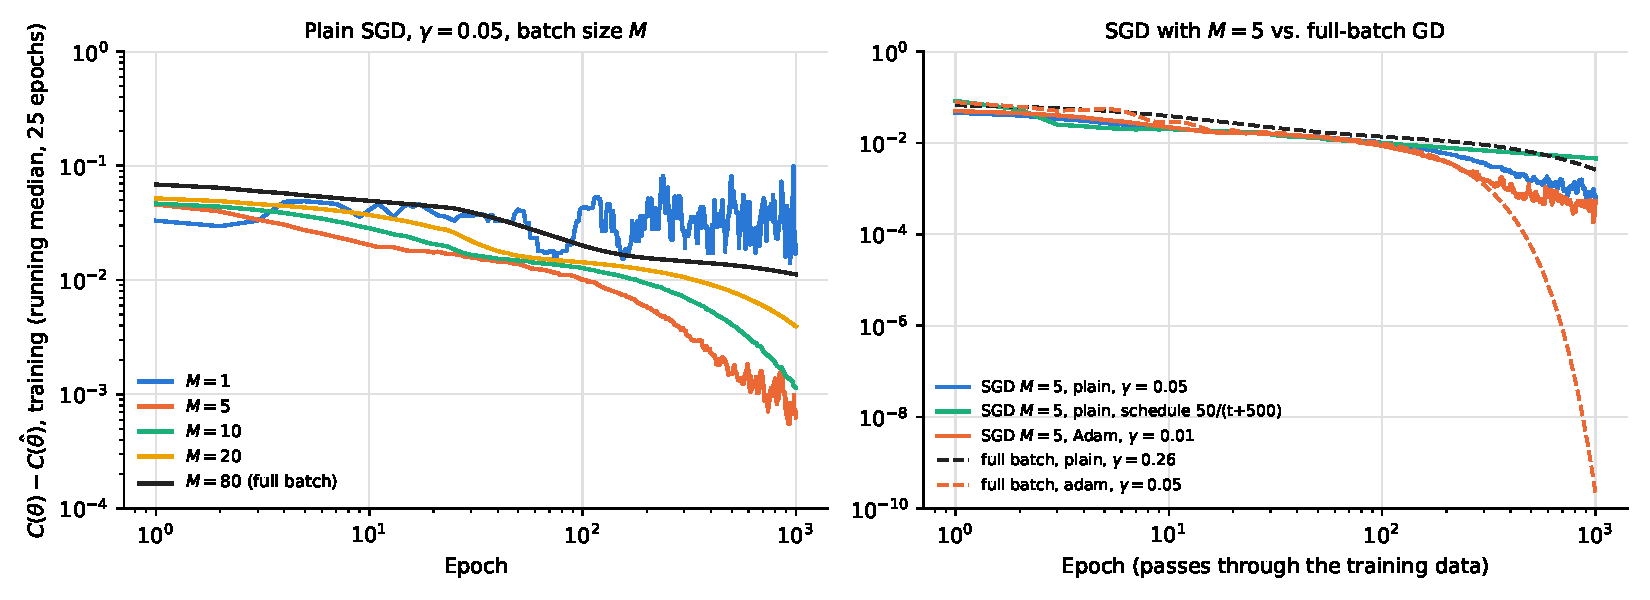
\includegraphics[width=0.85\textwidth]{h_sgd.pdf}
    \caption{SGD for OLS, degree 6, seed 42: training cost above the closed-form minimum against epochs (running median over 25 epochs for SGD). Left: plain SGD with $\gamma = 0.05$ for batch sizes $M$ ($M = 80$ is full batch). Right: SGD with $M = 5$ (constant rate, decaying schedule, Adam) against full-batch gradient descent, per pass through the data.}
    \label{fig:h_sgd}
\end{figure*}

\subsection{Final model selection}\label{sec:res_final}

Table~\ref{tab:i_selected} summarises the models chosen by cross-validation (Sec.~\ref{sec:resampling}), and Fig.~\ref{fig:i_cv} shows the cross-validation error against degree with the best $\lambda$ at each degree. By the cross-validated error the best model is Ridge with a small penalty: median CV MSE 0.0149 at a median degree of 11.5, with $\lambda$ between $10^{-8}$ and $10^{-5}$, against 0.0158 for OLS at degree 10. On new data the methods are nearly equal, 0.0136--0.0141, or about $1.4\,\sigma^2$, and which method is best varies between the data sets (OLS in 6, Ridge in 7 and Lasso in 7 of 20). The differences between the medians, at most 0.0005, are small compared with the spread over data sets: the interquartile range of the MSE on new data is 0.0131--0.0146 for Ridge and 0.0132--0.0150 for OLS. For OLS, Ridge and Lasso the selected degree ranges from 8 to 16. From degree 8 on, the median cross-validation error of Ridge and Lasso stays between 0.0154 and 0.0186, and that of OLS between 0.017 and 0.021 up to degree 12 (Fig.~\ref{fig:i_cv}), so the minimum is poorly determined, as in Sec.~\ref{sec:res_cv}.

\begin{table}
    \centering
    \caption{Models selected by 5-fold cross-validation on the training part of each of 20 data sets ($n = 100$, $\sigma = 0.1$): median and range of the degree, median $\lambda$, and median CV MSE, test MSE and MSE on new data. Lasso$^*$: only $\lambda \geq 10^{-3}$ allowed.}
    \label{tab:i_selected}
    \begin{tabular}{lccccc}
        \toprule
        Method & Degree & $\lambda$ & CV & Test & New data \\
        \midrule
        OLS         & 10 (8--16)   & --                 & 0.0158 & 0.0155 & 0.0141 \\
        Ridge       & 11.5 (8--16) & $10^{-7}$          & 0.0149 & 0.0133 & 0.0136 \\
        Lasso       & 12 (8--16)   & $5.5\times10^{-6}$ & 0.0163 & 0.0139 & 0.0140 \\
        Lasso$^*$   & 11.5 (6--16) & $10^{-3}$          & 0.0207 & 0.0184 & 0.0185 \\
        \bottomrule
    \end{tabular}
\end{table}

\begin{figure}
    \centering
    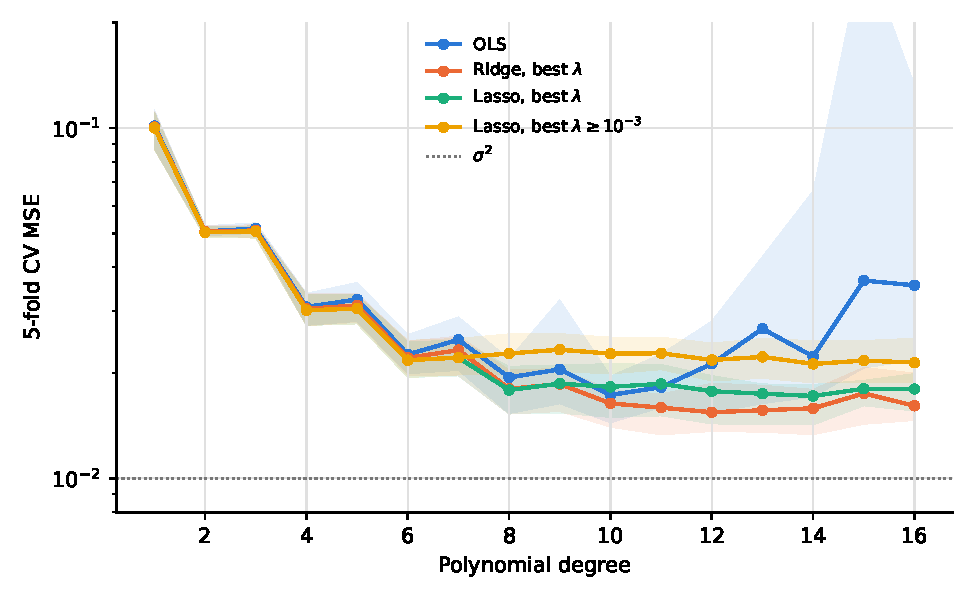
\includegraphics[width=\linewidth]{i_cv_methods.pdf}
    \caption{Median 5-fold CV MSE over 20 data sets against degree, with the best $\lambda$ at each degree for Ridge and Lasso; bands: interquartile range. For Lasso with $\lambda < 10^{-3}$ the solver has not converged at high degree (see text). $n = 100$, $\sigma = 0.1$.}
    \label{fig:i_cv}
\end{figure}

The methods differ at high degree. Up to degree 9 the curves of OLS, Ridge and Lasso differ by at most 12\,\%; above degree 11 the OLS error rises, to 0.036 at degree 16 with a wide band, while Ridge stays between 0.0154 and 0.0175 from degree 10 on. The strength of Ridge for this problem is that a small penalty removes the unstable directions (Sec.~\ref{sec:res_ridge}) and makes the result insensitive to the choice of degree, at practically no cost, and the solution has a closed form. OLS needs no $\lambda$, but its error depends strongly on getting the degree right.

For Lasso, cross-validation chose the smallest penalties in the grid ($10^{-6}$ in 10 of 20 data sets), and only 4 of the 20 selected models have a coefficient set to zero. At these penalties scikit-learn's coordinate descent often did not converge within $10^5$ iterations: 18 of the 20 selected Lasso fits stopped at the iteration limit, with a median duality gap of $8\times10^{-3}$ against a cost of $1.3\times10^{-2}$. What we call Lasso there is an early-stopped approximation, which regularises in its own way (Sec.~\ref{sec:res_sgd}), and its similarity to Ridge says little about the Lasso solution itself. If only $\lambda \geq 10^{-3}$ is allowed, where the solver converges (duality gap $2\times10^{-9}$), cross-validation chooses $\lambda = 10^{-3}$ in all 20 data sets. The models then have a median of 6 nonzero coefficients (16 of 20 have at least one zero), but the error on new data rises to 0.0185. For this problem the sparsity of Lasso is thus not an advantage: a good polynomial approximation of Runge's function needs many terms, and a penalty large enough to remove terms also adds bias. Its weaknesses here are the lack of a closed form and a slow solver when the columns are collinear.

\begin{table}
    \centering
    \caption{Bootstrap decomposition at degree 14 with the median selected penalties, 100 bootstrap samples, median over 20 data sets. Bias$^2$ is measured against the true $f$.}
    \label{tab:i_bootstrap}
    \begin{tabular}{lccc}
        \toprule
        Method & Error & Bias$^2$ & Variance \\
        \midrule
        OLS                                     & 0.102  & $8.0\times10^{-3}$ & 0.087 \\
        Ridge, $\lambda = 10^{-7}$              & 0.036  & $3.1\times10^{-3}$ & 0.024 \\
        Lasso, $\lambda = 5.5\times10^{-6}$     & 0.024  & $4.0\times10^{-3}$ & 0.013 \\
        Lasso, $\lambda = 10^{-3}$              & 0.021  & $8.9\times10^{-3}$ & 0.0023 \\
        \bottomrule
    \end{tabular}
\end{table}

In terms of the bias--variance decomposition, a higher degree in OLS attacks the bias: the bias against $f$ falls with the degree (Sec.~\ref{sec:res_bootstrap}). Ridge and Lasso attack the variance. At degree 14 the variance falls from 0.087 for OLS to 0.024 with Ridge ($\lambda = 10^{-7}$) and to 0.0023 with the converged Lasso ($\lambda = 10^{-3}$), see Table~\ref{tab:i_bootstrap}. For the converged Lasso the price is visible in the bias, $8.9\times10^{-3}$ against $3.1\times10^{-3}$ for Ridge. The bias of OLS, $8.0\times10^{-3}$, is not a real bias but the effect of a few extreme bootstrap fits on the mean prediction (Sec.~\ref{sec:res_bootstrap}). The numbers thus support the reading that the penalties trade variance for bias, with $\lambda$ setting the balance. At degree 14 the bootstrap ranks the converged Lasso best, unlike cross-validation; since the bootstrap overestimates the variance (Sec.~\ref{sec:res_cv}), it favours strong penalties.

% =====================================================================
% IV. CONCLUSION
% LLM declaration: text level 3; see Appendix "Use of AI/LLM tools".
% =====================================================================

\section{Conclusion}\label{sec:conclusion}

For OLS the test error of Runge's function falls with the polynomial degree until the variance takes over, and where that happens depends on the data: the best degree rose from 6 to 20 when $n$ went from 30 to 1000, and fell when the noise increased. The largest errors came from a few data sets where the model had to extrapolate or bridge a gap near the edges, so a single split, or the mean over many, can give a misleading picture. Ridge shrinks the directions of the design matrix with small singular values, which here contain mostly noise. With $n = 100$ it did not improve on OLS at the best fixed degree, but it removed the blow-up at high degree, and with $n = 30$ it gave the lowest error. The bootstrap split the error into bias and variance, with the variance overtaking the measured bias from degree 11 for $n = 100$, but it overestimated the error at high degree because each bootstrap sample contains only about 63\,\% distinct points; cross-validation followed the true error closely. In the final comparison by cross-validation, Ridge with a small penalty was best (0.0149 against 0.0158 for OLS), mainly because it keeps the variance down at high degree, but the differences between the methods were small compared with the differences between data sets. For the optimisation, the largest usable learning rate of plain gradient descent is set by the steepest curvature and the number of iterations by the flattest. Momentum gave the largest speed-up (601 against 11\,834 iterations), and Adam reached the criterion for every learning rate we tested, while RMSProp and Adam with a constant learning rate did not settle exactly at the minimum. Gradient descent with subgradients approached the Lasso solution when the step was small enough, but never gave exact zeros. With only 80 training points, stochastic gradient descent reached a moderate accuracy about as fast as full-batch gradient descent but did not settle as low, so it gave no clear advantage.

Several results are specific to our setup: one function in one dimension, uniformly drawn $x$ values, and one noise model. Many of our references, such as the error on new data and the bias measured against $f$, are possible only because $f$ is known. The resampling studies used 20 data sets, and the gradient-descent experiments one data set at degree 6, so the exact numbers there carry noticeable uncertainty. The median, which we used throughout, hides the extreme cases that a single real data set may well be. At high degree the bootstrap estimate of the bias is contaminated by a few extreme fits. Finally, scikit-learn's Lasso solver did not converge for small penalties at high degree, so our conclusions about Lasso with small penalties are uncertain; with the penalties where it converged, Lasso was clearly worse than Ridge.

Natural next steps would be to sample $x$ at Chebyshev nodes, which are denser near the edges, or to use an orthogonal polynomial basis, to reduce both the oscillations and the collinearity of the columns; to use a Lasso solver that converges for small penalties, to settle the comparison with Ridge; and to test decaying learning rates for Adam and stochastic gradient descent on a problem with many more data points, where stochastic gradient descent is expected to pay off.

% =====================================================================
% APPENDIX: supplementary figures and declaration of AI/LLM use
% =====================================================================

\appendix

\section{Supplementary figures}\label{app:figures}

\begin{figure}[h]
    \centering
    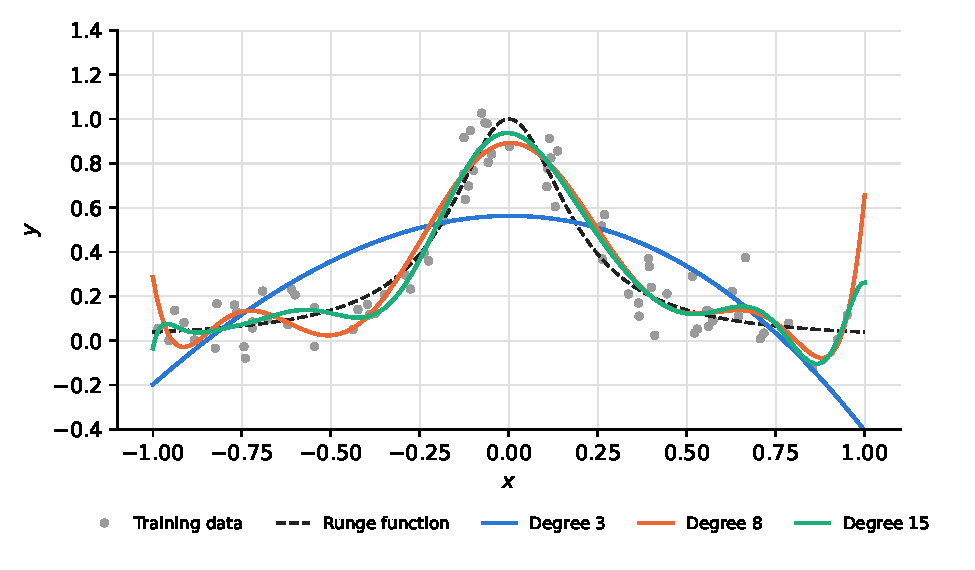
\includegraphics[width=\linewidth]{a_fits.pdf}
    \caption{Training data for seed 42, Runge's function, and OLS fits of degree 3, 8 and 15. The last training point is at $x = 0.951$; beyond it the degree-8 fit rises to 0.655 at $x = 1$, where $f(1) = 0.038$.}
    \label{fig:a_fits}
\end{figure}

\begin{figure*}
    \centering
    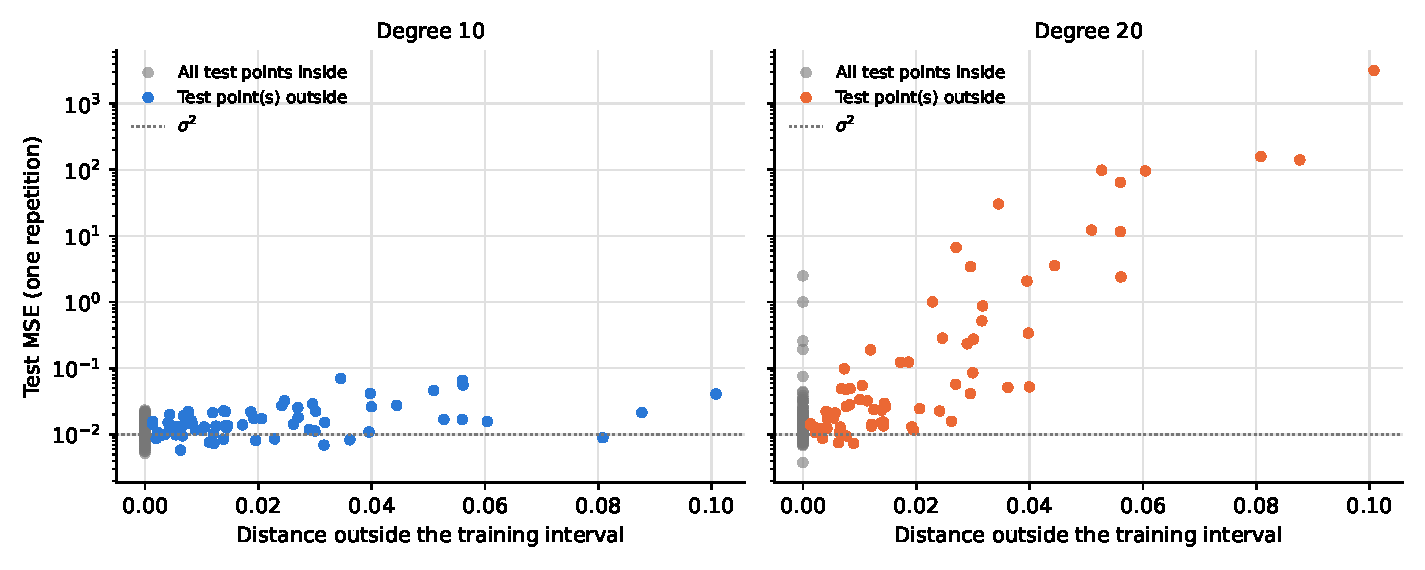
\includegraphics[width=0.85\textwidth]{a_extrapolation.pdf}
    \caption{Test MSE of each of the 200 repetitions against how far the test points reach outside the interval covered by the training points, for degree 10 (left) and 20 (right). Grey: all test points inside the training interval. $n = 100$, $\sigma = 0.1$.}
    \label{fig:a_extrapolation}
\end{figure*}

\section{Use of AI/LLM tools}\label{app:llm}

\paragraph*{Tools used.} Claude (Opus 5.5), accessed through claude.ai including its code-execution workspace, September 2026. Claude was also used as a tutor for the theory; the understanding this gave is not declared separately.

\paragraph*{Text.} Contribution levels as defined in the course guidelines.

\begin{table}[h]
    \centering
    \begin{tabular}{lc}
        \toprule
        Section & Level \\
        \midrule
        Abstract & 3 \\
        Introduction & 3 \\
        Methods & 3 \\
        Results and discussion & 3 \\
        Conclusion & 3 \\
        Appendix A (figure captions) & 3 \\
        Appendix B (this declaration) & 3 \\
        \bottomrule
    \end{tabular}
\end{table}

\emph{Level 3 note.} The text was drafted by Claude from our dialogue about the methods and the results. For the results, we interpreted the figures and the logged output of the code ourselves first; Claude corrected our interpretation and drafted the text from it. We read, corrected and approved all sections, and statements we could not explain ourselves were simplified or removed. Every number in the text was checked against the logged output of the code in a separate pass by Claude.

\paragraph*{Code.} Contribution levels as defined in the course guidelines. Every function and class carries an \texttt{LLM-assisted} tag in its docstring that refers to the note at the top of its file.

\begin{table}[h]
    \centering
    \begin{tabular}{lcp{0.55\linewidth}}
        \toprule
        File & Level & Description \\
        \midrule
        \texttt{common.py} & 4 & Data, design matrix, scaling, OLS and Ridge solvers, scikit-learn Lasso, error measures, bootstrap, scikit-learn wrapper. Written by Claude from choices agreed with the authors. \\
        \texttt{optim.py} & 4 & Cost, gradients (analytic and JAX), update rules, gradient descent and SGD, following the course's reference implementation. Written by Claude. \\
        \texttt{main.py} & 4 & One function per project part, figures and logged output. Written by Claude from the experiments agreed with the authors. \\
        \texttt{tests.py} & 4 & Unit tests. Written by Claude; the checks were chosen together with the authors. \\
        \bottomrule
    \end{tabular}
\end{table}

The results were first produced by running the code in Claude's code-execution workspace and then reproduced by running it locally; the numbers in this report are from the local run. The code was tested against scikit-learn, JAX and the closed-form solutions (Sec.~\ref{sec:validation}), and the choices behind the experiments (seeds, repetitions, grids, what to compare) were discussed and agreed on before the code was written.


\bibliographystyle{apsrev4-1}
\bibliography{refs}
\end{document}
